\documentclass[11pt,a4paper,oneside]{report}
\usepackage[utf8]{inputenc}
\usepackage[T1]{fontenc}
\usepackage[french]{babel}
\usepackage{lmodern}
\usepackage[a4paper,margin=2.5cm]{geometry}
\usepackage{microtype}
\usepackage{graphicx}
\usepackage{tikz}
\usetikzlibrary{calc}
\usepackage{booktabs,longtable,tabularx,array}
\usepackage{pdflscape,adjustbox}
\usepackage{enumitem}
\usepackage[table]{xcolor}
\usepackage{hyperref}
\usepackage{fancyhdr}
\usepackage{setspace}
\usepackage{titlesec}
\usepackage{caption}
\usepackage{float}
\usepackage{geometry}
\usepackage{colortbl}

\newcolumntype{L}[1]{>{\raggedright\arraybackslash}p{#1}}
\newcolumntype{C}[1]{>{\centering\arraybackslash}p{#1}}
\definecolor{bleuNuit}{HTML}{062B58}
\definecolor{orangeECSR}{HTML}{FF6A12}
\definecolor{grisRoute}{HTML}{69758B}
\definecolor{bleuECSR}{HTML}{174A74}
\definecolor{vertECSR}{HTML}{438259}
\hypersetup{colorlinks=true,linkcolor=bleuECSR,urlcolor=bleuECSR,pdftitle={Document écrit CCP2 ECSR}}
\titleformat{\chapter}[display]{\normalfont\huge\bfseries\color{bleuECSR}}{\chaptername\ \thechapter}{12pt}{\Huge}
\titleformat{\section}{\Large\bfseries\color{vertECSR}}{\thesection}{1em}{}
\pagestyle{fancy}\fancyhf{}\fancyhead[L]{\small Document écrit CCP2 -- TP ECSR}\fancyhead[R]{\small Action de sensibilisation}\fancyfoot[C]{\thepage}
\setlength{\headheight}{15pt}
\onehalfspacing
% Remplacer le texte-guide lorsque les faits et justificatifs sont disponibles.
\newcommand{\texteguide}[1]{\par\medskip\noindent\textcolor{gray}{\textit{[À compléter : #1]}}\par\medskip}
% ============================================
% PAGE DE GARDE -- TEXTES MODIFIABLES
% Changer les textes ci-dessous puis recompiler main.tex.
% ============================================
\newcommand{\TitreCertification}{TITRE PROFESSIONNEL}
\newcommand{\SigleFormation}{ECSR}
\newcommand{\BlocCertification}{CCP2}
\newcommand{\TitreMemoireLigneUn}{Sur la route}
\newcommand{\TitreMemoireLigneDeux}{du chantier}
\newcommand{\SousTitreMemoire}{Distracteurs au volant et risques professionnels}
\newcommand{\DescriptionMemoireLigneUn}{Action de sensibilisation aux risques routiers}
\newcommand{\DescriptionMemoireLigneDeux}{professionnels auprès de stagiaires plombiers}
\newcommand{\AxeUnTitre}{PÉDAGOGIE}
\newcommand{\AxeUnDescription}{Transmettre et\\faire progresser}
\newcommand{\AxeDeuxTitre}{SÉCURITÉ\\ROUTIÈRE}
\newcommand{\AxeDeuxDescription}{Prévenir les risques,\\sauver des vies}
\newcommand{\AxeTroisTitre}{RÉGLEMENTATION}
\newcommand{\AxeTroisDescription}{Appliquer et faire\\respecter les règles}
\newcommand{\AxeQuatreTitre}{MOBILITÉ\\RESPONSABLE}
\newcommand{\AxeQuatreDescription}{Former à une conduite\\citoyenne et durable}
\newcommand{\LieuMemoire}{AFPA NICE}
\newcommand{\FormationPublic}{Métiers du bâtiment :\\Plombier}
\newcommand{\SignatureMemoire}{Des déplacements professionnels\\plus sûrs et responsables}

% ======= CHOIX DES COUVERTURES =======
% Pour comparer les deux modèles, laisser les deux à true.
% Pour n'en garder qu'une, remplacer true par false sur l'autre ligne.
\newif\ifCouvertureEditable
\CouvertureEditablefalse
\newif\ifCouvertureImage
\CouvertureImagetrue
% =====================================
\begin{document}
\ifCouvertureEditable
  % Mise en page 100% native TikZ, couverture A4 portrait.
% Seules les photos et les marques institutionnelles sont des images.
\newgeometry{margin=0pt}
\begin{titlepage}
\thispagestyle{empty}
\begin{tikzpicture}[remember picture,overlay,x=1mm,y=1mm]
\coordinate (SW) at (current page.south west);
\begin{scope}[shift={(SW)}]
\fill[white] (0,0) rectangle (210,297);
% Bandeaux supérieurs
\fill[bleuNuit] (5,283) rectangle (29,284);
\fill[bleuNuit] (181,283) rectangle (205,284);
\node[anchor=center,inner sep=0] at (69,282) {
\includegraphics[width=73mm]{images/logo_aftral.png}};
\draw[bleuNuit,line width=.4pt] (113,274)--(113,292);
\node[anchor=center,inner sep=0] at (146,282) {
\includegraphics[width=42mm]{images/logo_afpa.png}};
% Entête académique
\draw[bleuNuit!40,line width=.45pt] (18,264)--(57,264);
\draw[bleuNuit!40,line width=.45pt] (153,264)--(192,264);
\node[font=\fontsize{16}{19}\selectfont\bfseries,color=bleuNuit] at (105,265) {\TitreCertification};
\node[font=\fontsize{16}{19}\selectfont\bfseries,color=bleuNuit] at (105,255) {\SigleFormation\quad\textcolor{orangeECSR}{$\bullet$}\quad\BlocCertification};
\fill[orangeECSR] (91,246) rectangle (119,247.3);
% Grand titre
\node[anchor=center,font=\fontsize{38}{43}\selectfont\bfseries,color=bleuNuit] at (96,228) {\TitreMemoireLigneUn};
\node[anchor=center,font=\fontsize{38}{43}\selectfont\bfseries,color=bleuNuit] at (96,211) {\TitreMemoireLigneDeux};
% Route stylisée à droite du titre
\draw[orangeECSR,line width=2mm] (164,240) .. controls (201,226) and (189,216) .. (180,209);
\draw[grisRoute,line width=6mm] (161,235) .. controls (196,225) and (185,217) .. (174,209);
\draw[white,line width=.6mm,dash pattern=on 2mm off 2mm] (162,234) .. controls (191,224) and (180,217) .. (174,212);
% Bandeau orange, texte dynamique
\fill[grisRoute] (25,188) -- (33,201) -- (39,201) -- (31,188) -- cycle;
\fill[orangeECSR] (36,188) -- (44,201) -- (194,201) -- (186,188) -- cycle;
\node[anchor=center,text=white,font=\fontsize{20}{23}\selectfont\itshape] at (111,194.5) {\SousTitreMemoire};
\fill[orangeECSR] (91,182) rectangle (119,182.8);
\node[font=\fontsize{13}{15}\selectfont\itshape,color=bleuNuit] at (105,174) {\DescriptionMemoireLigneUn};
\node[font=\fontsize{13}{15}\selectfont\itshape,color=bleuNuit] at (105,167) {\DescriptionMemoireLigneDeux};
% Graphisme chantier à gauche, stylisé en vecteurs
\begin{scope}[opacity=.28]
\fill[grisRoute!40] (5,90) -- (5,132) -- (37,132) -- (37,90) -- cycle;
\foreach \yy in {99,108,117,126}{\draw[bleuNuit,line width=.5pt] (5,\yy)--(37,\yy);}
\foreach \xx in {11,20,29}{\draw[bleuNuit,line width=.5pt] (\xx,90)--(\xx,132);}
\draw[bleuNuit,line width=.8pt] (17,131)--(20,152)--(23,131) (20,152)--(55,148) (20,152)--(7,143);
\draw[bleuNuit,line width=.5pt] (20,148)--(51,148) (42,148)--(42,137);
\end{scope}
% photo recadrée / masque polygonal incliné
\begin{scope}
\clip (74,161) -- (203,161) -- (203,94) -- (173,88) -- (14,88) -- (75,161) -- cycle;
\node[inner sep=0,anchor=south west] at (23,88) {
\includegraphics[width=187mm,height=78mm]{images/photo_conducteur.png}};
\end{scope}
% Masques d'angles blancs et accents orange
\fill[orangeECSR] (10,80)--(16,80)--(42,111)--(36,111)--cycle;
\fill[orangeECSR] (183,96)--(200,115)--(200,110)--(188,96)--cycle;
% Axes / pictogrammes dessinés en TikZ
\draw[bleuNuit!40,line width=.45pt] (53,54)--(53,77);
\draw[bleuNuit!40,line width=.45pt] (105,54)--(105,77);
\draw[bleuNuit!40,line width=.45pt] (157,54)--(157,77);
% pédagogie : mortier et pompon
\draw[bleuNuit,line width=.8pt] (23,72)--(34,77)--(45,72)--(34,67)--cycle;
\draw[bleuNuit,line width=.8pt] (28,70)--(28,65) .. controls (34,62) and (40,65) .. (40,70);
\draw[bleuNuit,line width=.8pt] (45,72)--(45,65);
% bouclier
\draw[orangeECSR,line width=.9pt] (81,77)--(88,80)--(95,77)--(95,70) .. controls (92,66) and (89,63) .. (88,63) .. controls (85,66) and (81,69) .. (81,70)--cycle;
\draw[orangeECSR,line width=.9pt] (84,71)--(87,68)--(92,74);
% balance
\draw[bleuNuit,line width=.8pt] (131,77)--(131,64) (122,73)--(140,73) (125,77)--(137,77);
\draw[bleuNuit,line width=.7pt] (124,73)--(120,66)--(128,66)--cycle (138,73)--(134,66)--(142,66)--cycle;
\draw[bleuNuit,line width=.8pt] (124,63)--(138,63);
% feuille
\draw[vertECSR,line width=.85pt] (181,64) .. controls (173,73) and (185,80) .. (190,80) .. controls (193,68) and (188,63) .. (181,64);
\draw[vertECSR,line width=.75pt] (178,60)--(188,75);
% 4 thèmes
\node[anchor=north,align=center,text width=48mm,font=\fontsize{10}{11}\selectfont\bfseries,color=bleuNuit] at (29,61) {\AxeUnTitre};
\node[anchor=north,align=center,text width=48mm,font=\fontsize{8}{10}\selectfont\itshape,color=bleuNuit] at (29,47) {\AxeUnDescription};
\node[anchor=north,align=center,text width=48mm,font=\fontsize{10}{11}\selectfont\bfseries,color=bleuNuit] at (80,61) {\AxeDeuxTitre};
\node[anchor=north,align=center,text width=48mm,font=\fontsize{8}{10}\selectfont\itshape,color=bleuNuit] at (80,47) {\AxeDeuxDescription};
\node[anchor=north,align=center,text width=48mm,font=\fontsize{10}{11}\selectfont\bfseries,color=bleuNuit] at (131,61) {\AxeTroisTitre};
\node[anchor=north,align=center,text width=48mm,font=\fontsize{8}{10}\selectfont\itshape,color=bleuNuit] at (131,47) {\AxeTroisDescription};
\node[anchor=north,align=center,text width=48mm,font=\fontsize{10}{11}\selectfont\bfseries,color=bleuNuit] at (183,61) {\AxeQuatreTitre};
\node[anchor=north,align=center,text width=48mm,font=\fontsize{8}{10}\selectfont\itshape,color=bleuNuit] at (183,47) {\AxeQuatreDescription};
\draw[bleuNuit,line width=.5pt] (12,31)--(198,31);
% bande d'information inférieure
\node[anchor=west,font=\fontsize{10}{12}\selectfont\bfseries,color=bleuNuit] at (10,21) {\LieuMemoire};
\draw[bleuNuit!50] (59,15)--(59,26);
\node[anchor=center,align=center,font=\fontsize{9}{11}\selectfont,color=bleuNuit] at (105,20) {\FormationPublic};
\draw[bleuNuit!50] (146,15)--(146,26);
\node[anchor=center,align=center,font=\fontsize{9}{11}\selectfont\itshape,color=bleuNuit] at (175,20) {\SignatureMemoire};
\fill[bleuNuit] (0,0)--(210,0)--(210,10)--(163,3)--(0,4)--cycle;
\fill[orangeECSR] (125,0)--(210,0)--(210,9)--(166,2)--cycle;
\fill[bleuNuit] (0,0)--(210,0)--(210,6)--(163,1)--(0,3)--cycle;
\end{scope}
\end{tikzpicture}
\end{titlepage}
\restoregeometry
\clearpage

\fi
\ifCouvertureImage
  % Deuxième couverture : image fixe avec promotion 2026-2027.
% Ne modifie pas la couverture TikZ native.
\newgeometry{margin=0pt}
\begin{titlepage}
  \thispagestyle{empty}
  \begin{tikzpicture}[remember picture,overlay]
    \node[inner sep=0,anchor=center] at (current page.center) {%
      
\includegraphics[width=\paperwidth,height=\paperheight]{images/couverture_image_session_2026_2027.png}%
    };
  \end{tikzpicture}
\end{titlepage}
\restoregeometry

\fi
\pagenumbering{roman}
\tableofcontents
\clearpage
\pagenumbering{arabic}
\chapter{Introduction}

\section{Présentation personnelle}
Je suis Sam FOKAM WABO, stagiaire en formation au titre professionnel d'enseignant de la conduite et de la sécurité routière (ECSR). Mon parcours professionnel antérieur, notamment dans le développement informatique, m'a appris à structurer un projet, à rechercher des informations, à analyser des besoins et à documenter les décisions prises. Dans le cadre de ma reconversion vers l'enseignement de la conduite, je souhaite mobiliser cette méthode de travail au service d'une pédagogie active et de la prévention des risques routiers.

Le certificat de compétences professionnelles n\textsuperscript{o} 2 (CCP2) porte sur la sensibilisation de l'ensemble des usagers de la route à l'adoption de comportements sûrs et respectueux de l'environnement. Il ne s'agit pas seulement de transmettre des règles : l'enjeu est de comprendre un public, de construire une intervention pertinente, de l'animer puis d'en évaluer les effets et sa propre pratique.

Cette action est conduite en binôme avec Manane SADIK, également stagiaire en formation ECSR. Notre commanditaire est le centre AFPA de Nice, représenté dans nos échanges par Mme Muriel LIÉGEOIS, responsable de formation du centre AFPA Nice/Cannes. L'intervention, prévue le 4 décembre 2026, s'adresse à un groupe de stagiaires en formation de plomberie. Nous avons retenu le thème général « Sur la route du chantier », centré sur l'alcool et les distracteurs pendant les déplacements professionnels.

\section{Démarche et périmètre du présent mémoire}
Ce mémoire retrace une démarche progressive : recherche d'un commanditaire, clarification de sa demande, enquête auprès du public, hiérarchisation des besoins, conception d'une réponse et recherche de ressources pédagogiques. Il est rédigé à la première personne pour rendre explicites mes initiatives, mes choix et les analyses effectuées conjointement avec ma collègue.

\textbf{État du dossier au 11 novembre 2026 :} la phase de diagnostic et une première version de la préparation pédagogique sont documentées. L'action du 4 décembre n'a pas encore eu lieu. Ses résultats, les retours des participants et l'analyse réflexive ne sont donc pas anticipés : ils seront rédigés après l'intervention, sur la base d'observations et de pièces vérifiables.

\chapter{Choix et présentation du commanditaire}

\section{Choix du commanditaire}
Le 3 juillet 2026, lors de la kermesse à l'école Rancher de Nice, ou sont scolarisés mes enfants, j'ai échangé avec la directrice de l'établissement Mme Hélène Fouassier au sujet d'une éventuelle intervention de sécurité routière auprès d'élèves de CM2. Un accord de principe a été évoqué pour l'année scolaire 2026--2027 le même jour. J'ai également pris contact avec un responsable d'une entreprise de sécurité présente lors de l'événement ; cette piste n'a pas donné de suite favorable.

Ma collègue Manane SADIK m’a parlé de l’AFPA de Nice, après avoir obtenu cette information par l’intermédiaire d’une de ses connaissances. Cette piste nous a intéressés, car elle nous permettait de nous adresser à un public adulte confronté à des déplacements liés à la formation et à la future activité professionnelle. Nous avons donc choisi d’explorer cette possibilité afin de travailler sur des situations concrètes de risque routier. Ce choix ne remet pas en cause l’intérêt d’une sensibilisation auprès des enfants, mais il correspondait davantage à notre volonté de travailler sur des comportements et des décisions observables dans un contexte professionnel.

L'AFPA de Nice nous a paru pertinente en raison de la diversité de ses formations et de la possibilité d'aborder les trajets domicile--formation, mais aussi les futurs déplacements entre entreprise, fournisseurs, clients et chantiers. Ce dernier contexte constituait d'abord une \emph{hypothèse de pertinence}, à préciser avec le commanditaire et les stagiaires.

\section{Premier courriel de contact}
Le 3 septembre 2026, nous nous sommes rendus à l'AFPA de Nice en fin de journée. N'ayant pas pu rencontrer directement les responsables, nous avons contacté l'accueil par téléphone pour présenter notre proposition et demander qu'elle soit transmise à la direction.

Le 9 septembre 2026 à 15\,h\,33, nous avons adressé à Mme Muriel LIÉGEOIS un courriel intitulé « \textbf{Proposition d'une action gratuite de sensibilisation à la sécurité routière} ». Nous y présentions le cadre du TP ECSR, la gratuité de l'intervention et une durée envisagée d'environ deux heures.

Nous avons surtout souligné que nous ne souhaitions \textbf{pas imposer un thème} : notre intention était de recueillir les attentes de l'AFPA, d'identifier les éventuelles problématiques et de construire une réponse adaptée au public. Le courriel proposait des pistes ouvertes (fatigue, téléphone, vitesse, alcool, stupéfiants, partage de la route, risques professionnels ou éco-conduite), sans les présenter comme des problèmes établis au sein du centre.

Cette prise de contact poursuivait un double objectif : proposer une action utile aux participants et exercer, dans un cadre réel, les compétences attendues d'un futur enseignant de la conduite.

\section{Entretien téléphonique}
Le 10 septembre 2026 à 11\,h\,23, Mme LIÉGEOIS a répondu favorablement à notre proposition et nous a invités à l'appeler pour en discuter. J'ai donné suite à cette invitation par téléphone. Cet échange a ouvert la phase de clarification du besoin et confirmé l'intérêt d'un questionnaire destiné au commanditaire.

Le 11 septembre, j'ai annoncé l'envoi de ce questionnaire mais omis la pièce jointe. Mme LIÉGEOIS l'a signalé le même jour. Le 23 septembre à 15\,h\,59, j'ai transmis le document avec des excuses. Cette correction fait partie du suivi administratif du projet ; elle rappelle l'importance de contrôler les pièces jointes avant l'envoi d'un document de travail.

\section{Présentation du commanditaire}
L'AFPA est un organisme de formation professionnelle d'adultes. Dans notre projet, l'interlocutrice du commanditaire est Mme Muriel LIÉGEOIS, responsable de formation au centre AFPA Nice/Cannes, situé dans les Alpes-Maritimes.


Le 19 novembre 2026, Mme LIÉGEOIS nous a transmis un organigramme anonymisé du centre AFPA de Nice. Ce document montre une organisation structurée autour d'une direction de centre, de responsables de formation et de fonctions supports. Pour notre action, il confirme que Mme LIÉGEOIS occupe une position d'interface entre les stagiaires, l'équipe pédagogique et l'organisation du site. Cette place dans l'organigramme éclaire son rôle dans notre projet : accueillir la demande, faciliter la coordination de l'action et orienter les échanges vers les interlocuteurs compétents lorsque cela est nécessaire.

\begin{figure}[H]
  \centering
  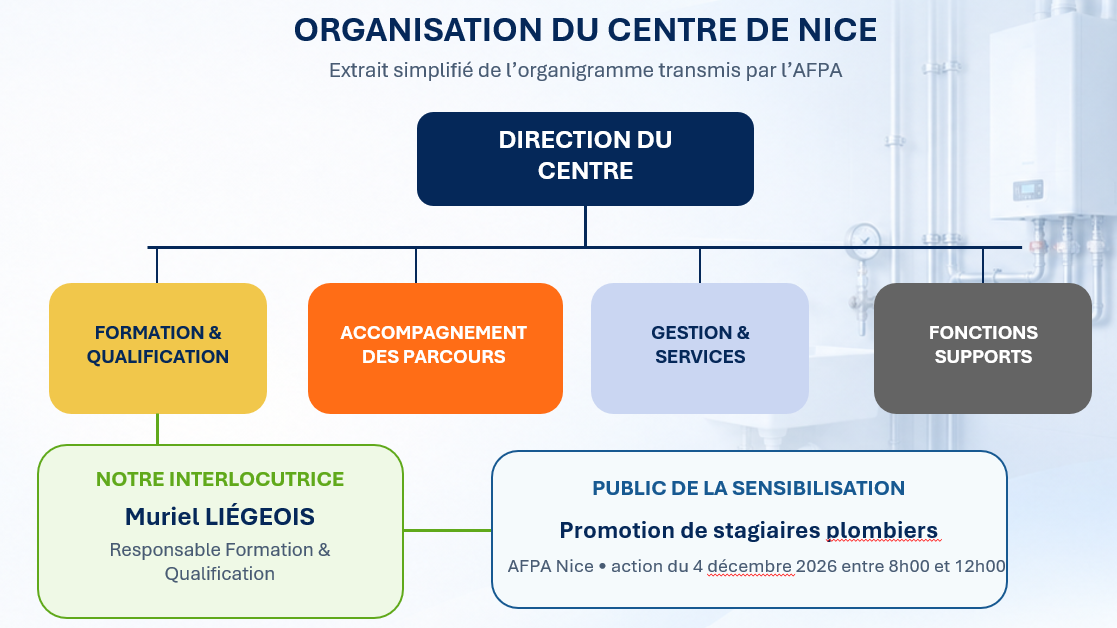
\includegraphics[width=0.72\textwidth,keepaspectratio]{images/organisation_afpa_nice_simplifiee.png}
  \caption{Organisation simplifiée du centre AFPA de Nice, à partir de l'organigramme transmis par le commanditaire.}
  \label{fig:organisation-afpa-nice}
\end{figure}

\section{Entretien avec le commanditaire}
Le 28 septembre, Mme LIÉGEOIS nous a retourné son questionnaire de recueil des besoins et a proposé une date d'intervention. Afin de dépasser la seule lecture du formulaire, j'ai sollicité le même jour un rendez-vous pour préciser le profil des participants et les objectifs attendus. Mme LIÉGEOIS a confirmé un entretien le \textbf{jeudi 1\textsuperscript{er} octobre 2026 à 15\,h}, et nous a adressé une invitation Outlook.

Au cours de cet échange, nous avons réexaminé le public et le format envisagés. Une première estimation d'environ quarante participants a été jugée peu compatible avec une animation participative. Le projet a été recentré sur un groupe d'environ dix à quinze stagiaires, appartenant à une promotion de plomberie et âgés approximativement de dix-huit à trente ans selon les informations fournies. Le statut individuel de conducteur et les habitudes de déplacement restaient à vérifier.

La date finalement proposée par le commanditaire est le \textbf{4 décembre 2026 entre 8h00 et 12h00}. Dans son message du 28 septembre, Mme LIÉGEOIS avait d'abord écrit « 4/11 » puis a explicitement corrigé cette erreur en précisant « 04/12 ». La correction est retenue dans notre chronologie.


\chapter{Diagnostic du public et choix du thème}
\section{Pourquoi interroger les stagiaires ?}

Le questionnaire du commanditaire nous a donné un premier cadre, mais il ne suffisait pas pour choisir un thème. Les risques cités concernaient l’établissement de manière générale et ne prouvaient pas que les stagiaires plombiers avaient les mêmes besoins.

Nous avons donc créé un questionnaire anonyme de trente questions destiné directement au groupe. Il abordait la situation de déplacement, la vitesse, le téléphone et les distracteurs, l’alcool, les stupéfiants, les médicaments, la ceinture et une dernière partie consacrée à la perception globale et aux attentes.

Les questions avaient trois objectifs simples : vérifier certaines connaissances, repérer des comportements déclarés et identifier des représentations pouvant influencer une décision. Plusieurs mises en situation ont été adaptées au métier de plombier : retard sur un chantier, appel d’un client, recherche d’adresse ou déplacement en véhicule utilitaire.

Le questionnaire a été transmis à Mme LIÉGEOIS le 26 octobre 2026. Après une relance le 29 octobre, nous avons reçu treize questionnaires exploitables. Les réponses sont anonymes et utilisées uniquement de manière collective.

\section{Méthode de lecture des réponses}

Pour l’analyse, j’ai séparé deux catégories :

— les connaissances et perceptions : réponse fausse, incertitude ou représentation pouvant conduire à sous-estimer un risque ;

— les comportements et situations à risque : comportement déclaré ou décision choisie dans une mise en situation.

Cette distinction est importante : une mauvaise réponse ne prouve pas un comportement dangereux, et un comportement déclaré ne permet pas d’affirmer qu’une infraction a été réellement commise.

Pour le graphique de synthèse, la partie H du questionnaire n’est pas utilisée dans le calcul car elle porte surtout sur les attentes et les thèmes que les stagiaires souhaitent aborder.

\section{Profil de déplacement du groupe}

Parmi les 13 répondants :

— 11/13 déclarent posséder le permis B ;

— 2/13 ne le possèdent pas ;

— 4/13 conduisent tous les jours ;

— 2/13 plusieurs fois par semaine ;

— 4/13 occasionnellement ;

— 3/13 ne conduisent jamais.

Le groupe est donc assez hétérogène. Je dois proposer une sensibilisation compréhensible aussi bien par les conducteurs réguliers que par les non-conducteurs ou futurs conducteurs.

\section{Deux besoins ressortent nettement}

La comparaison des six thèmes montre deux résultats principaux.

\begin{figure}[H]\centering
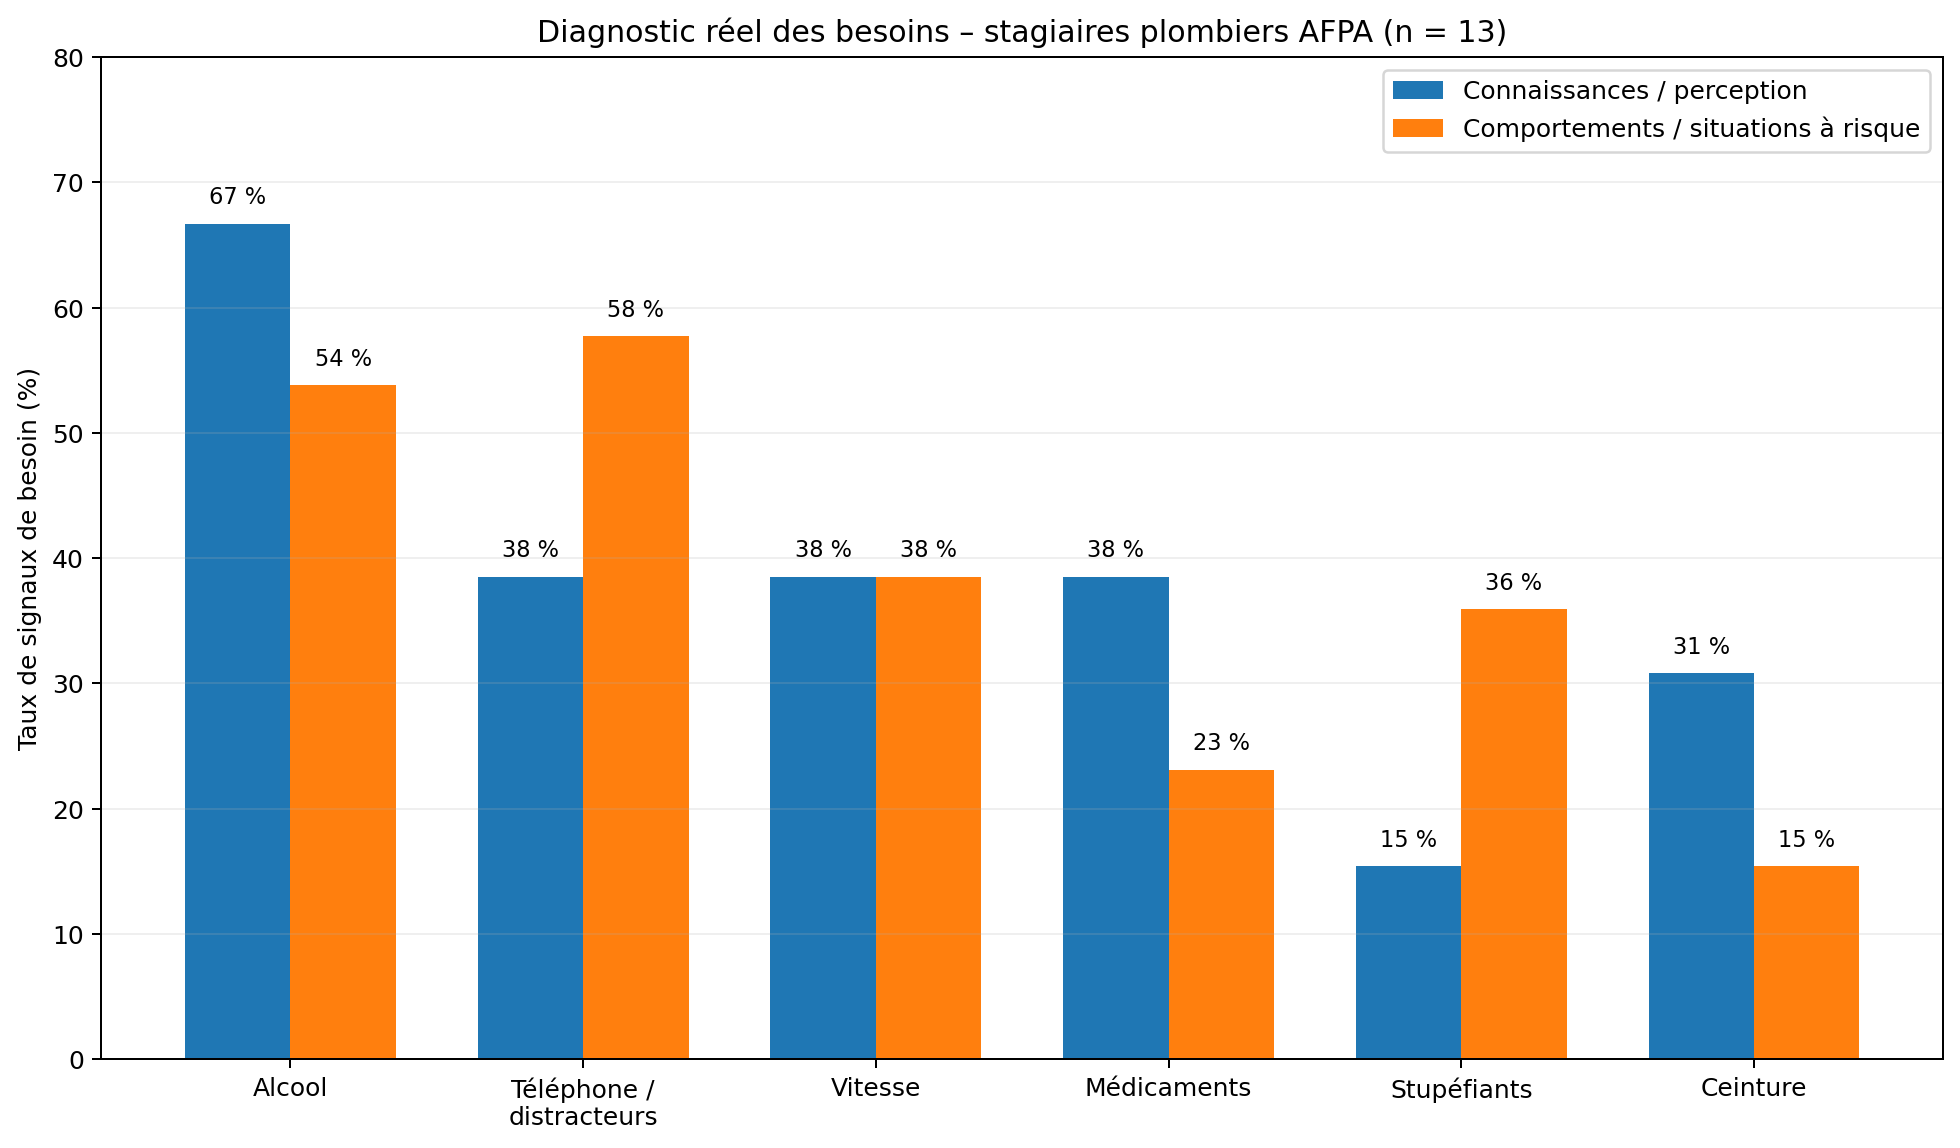
\includegraphics[width=0.92\textwidth]{images/diagnostic_afpa_13_repondants.png}
\caption{Signaux de besoin par thème pour les 13 répondants.}
\end{figure}

\begin{table}[H]
\centering\small
\caption{Lecture synthétique des réponses (n = 13)}
\begin{tabularx}{\textwidth}{@{}Xcc@{}}
\toprule
\rowcolor{bleuECSR}\textcolor{white}{\textbf{Thème}} & \textcolor{white}{\textbf{Connaissances / perception}} & \textcolor{white}{\textbf{Comportements / situations à risque}} \\
\midrule
Alcool & 69,23\,\% (9/13) & 53,85\,\% (7/13) \\
Téléphone / distracteurs & 38,46\,\% (5/13) & 61,54\,\% (8/13) \\
Vitesse & 38,46\,\% (5/13) & 38,46\,\% (5/13) \\
Médicaments & 38,46\,\% (5/13) & 23,08\,\% (3/13) \\
Stupéfiants & 15,38\,\% (2/13) & 38,46\,\% (5/13) \\
Ceinture de sécurité & 30,77\,\% (4/13) & 15,38\,\% (2/13) \\
\bottomrule
\end{tabularx}
\end{table}


\subsection{Alcool : surtout un besoin de connaissances et de perception}

L’alcool obtient le niveau le plus élevé dans la catégorie connaissances / perception : 69,23 \% (9/13). Le volet comportements / situations à risque atteint 53,85 \% (7/13).

Cela montre que l’alcool mérite une action de sensibilisation, notamment sur les effets, l’élimination et la confiance accordée à son propre ressenti. Comme nous travaillons en binôme, l’analyse détaillée de ce thème et sa réponse pédagogique sont développées par ma collègue Manane SADIK.

\subsection{Téléphone et distracteurs : surtout un besoin comportemental}

Pour le téléphone et les distracteurs, le résultat est différent : 38,46 \% (5/13) pour les connaissances et perceptions, mais 61,54 \% (8/13) pour les comportements et situations à risque. C’est le niveau comportemental le plus élevé des six thèmes.

Deux réponses m’ont particulièrement intéressé : 11/13 stagiaires savent qu’un dispositif mains libres ne supprime pas complètement le risque de distraction, mais 8/13 déclarent consulter une notification ou un message au volant au moins occasionnellement.

Ce décalage est important pour moi : connaître le danger ne suffit pas toujours à adopter la bonne décision. Dans le métier de plombier, cette situation peut se retrouver lors d’un appel client, d’un message du responsable, d’une recherche d’adresse ou d’un retard sur un chantier.

\chapter{Analyse de la demande et structuration de la réponse}

\section{Questionnaire pour le commanditaire}
Pour éviter de sélectionner un thème à partir de nos seules représentations, nous avons élaboré un questionnaire de recueil des besoins à destination de l'AFPA. Annoncé dès notre proposition du 9 septembre, il a été transmis en pièce jointe le 23 septembre 2026 après correction d'un premier envoi incomplet du 11 septembre.

Le document interrogeait notamment le public visé, son effectif, ses déplacements supposés, les situations de risque identifiées par le commanditaire, les attentes de l'établissement et les moyens matériels disponibles. Notre objectif était d'obtenir une première photographie du cadre de l'action, avant de la confronter aux caractéristiques effectives du public.

Mme LIÉGEOIS a renvoyé le questionnaire complété le 29 septembre, après un premier message du 28 septembre dans lequel la pièce jointe manquait. Le document renseigné a servi de support à notre rendez-vous du 1\textsuperscript{er} octobre.

\section{Réponses du commanditaire}
L'analyse du premier questionnaire a conduit à plusieurs décisions.
\begin{itemize}[leftmargin=*]
\item \textbf{Délimiter le public :} le projet, initialement ouvert à divers personnels et stagiaires, a été recentré sur une promotion de plomberie.
\item \textbf{Adapter l'effectif :} l'estimation initiale d'environ quarante personnes a été ramenée à une cible de dix à quinze, plus compatible avec les échanges et les manipulations en petits groupes.
\item \textbf{Vérifier les mobilités :} les modes de déplacement évoqués par le commanditaire concernaient l'établissement de manière générale et ne décrivaient pas nécessairement la promotion ciblée.
\item \textbf{Hiérarchiser les risques :} l'alcool, le téléphone, les stupéfiants, les médicaments et la banalisation des risques ont été évoqués comme pistes, sans que leur prévalence réelle soit établie.
\item \textbf{Identifier les contraintes :} l'action était envisagée dans les locaux du centre, avec des moyens de projection et un espace extérieur potentiellement mobilisable.
\end{itemize}

La réponse du commanditaire a donc fourni un \textbf{cadrage} utile, mais non un diagnostic suffisant. En particulier, les comportements attribués de manière générale à certains stagiaires de l'AFPA ne devaient pas être extrapolés à la nouvelle promotion.

\section{Questionnaire aux participants}
Nous avons conçu un second questionnaire anonyme destiné aux stagiaires de plomberie. Il comporte trente questions réparties en huit domaines : situation de déplacement ; vitesse ; téléphone et distracteurs ; alcool ; stupéfiants ; médicaments ; ceinture ; perception globale des risques.

Le choix de ces rubriques répondait à trois objectifs : établir quelques connaissances de base, recueillir des comportements déclarés et rechercher les représentations pouvant influencer les décisions. Plusieurs scénarios s'inscrivent dans l'univers professionnel du plombier : retard sur un chantier, appel d'un client, fin de journée ou déplacement en véhicule utilitaire.

Le questionnaire a été adressé à Mme LIÉGEOIS le \textbf{26 octobre 2026 à 11\,h\,49}. Elle a répondu le jour même qu'elle le ferait compléter dans la semaine. Nous avons effectué une relance le 29 octobre ; Mme LIÉGEOIS a indiqué qu'elle transmettrait les formulaires numérisés. Notre analyse repose finalement sur \textbf{treize réponses exploitables}, regroupées dans un fichier de données.

L'anonymat était annoncé aux stagiaires : aucune identité n'était demandée. Les réponses sont exploitées collectivement et ne servent ni à qualifier une personne ni à établir une infraction. Les questions relatives aux comportements reposent sur l'auto-déclaration, susceptible de biais de mémoire et de désirabilité sociale.

\section{Synthèse des réponses des participants}
\subsection{Méthode de traitement}
Nous avons rapproché les réponses individuelles des questions posées, puis compté les effectifs de réponses correctes, erronées ou révélatrices d'un risque. Le dénominateur utilisé est de treize répondants. Certaines questions, malgré leur formulation au singulier, ont accepté plusieurs réponses dans le formulaire numérique. Nous le signalons lorsque cela influe sur la lecture des résultats.

La distinction entre \emph{connaissances / perceptions} et \emph{comportements / intentions déclarés} est essentielle : une connaissance erronée n'est pas un comportement observé, et une intention ne constitue pas une preuve d'action réelle.

\subsection{Profil de déplacement du groupe}
\begin{itemize}[leftmargin=*]
\item \textbf{11/13} répondants déclarent posséder le permis B.
\item \textbf{2/13} ne le possèdent pas. 
\item \textbf{4/13} déclarent conduire tous les jours.
\item \textbf{2/13} plusieurs fois par semaine.
\item \textbf{4/13} occasionnellement.
\item \textbf{3/13} jamais. 

\end{itemize}

Ces résultats confirment que le groupe n'est pas homogène en matière d'expérience de conduite. Les situations pédagogiques doivent donc rester accessibles à tous les usagers, conducteurs actuels ou futurs.

\subsection{L'alcool : un besoin prioritaire en connaissances et en perception}
La figure~\ref{fig:diagnostic-afpa} met en évidence, pour l'alcool, le taux le plus élevé de \emph{signaux de besoin en connaissances et en perception} parmi les six thèmes étudiés : \textbf{69,23\,\% (9/13)}. Le volet \emph{comportements et situations à risque} atteint \textbf{53,85\,\% (7/13)}. Ces valeurs, issues de l'indicateur synthétique présenté sur la figure, montrent l'intérêt d'une sensibilisation sur cette problématique, sans constituer à elles seules une mesure d'alcoolémie ni une observation directe des conduites.

\begin{table}[htbp]
\centering\small
\caption{Indicateurs de synthèse de la figure~\ref{fig:diagnostic-afpa} : alcool (13 répondants)}
\begin{tabularx}{\textwidth}{@{}Xrr@{}}
\toprule
\rowcolor{bleuECSR}
\textcolor{white}{\textbf{Catégorie de signaux}} & \textcolor{white}{\textbf{Effectif affiché}} & \textcolor{white}{\textbf{Taux affiché}} \\
\midrule
Connaissances / perception & 9/13 & 69,23\,\% \\
Comportements / situations à risque & 7/13 & 53,85\,\% \\
\bottomrule
\end{tabularx}
\end{table}

Ces constats figurent dans notre diagnostic commun. Toutefois, afin d'approfondir chaque thème sans redondance, \textbf{l'analyse détaillée des réponses sur l'alcool et la réponse pédagogique correspondante seront développées dans le mémoire de ma collègue Manane SADIK}. Le présent mémoire se concentre sur les distracteurs, notamment sur les sollicitations téléphoniques pendant les déplacements professionnels des futurs plombiers.

\subsection{Le téléphone et les distracteurs : un besoin principalement comportemental}
Pour le téléphone et les distracteurs, la figure~\ref{fig:diagnostic-afpa} indique \textbf{38,46\,\% (5/13)} de signaux de besoin en \emph{connaissances et perception}, contre \textbf{61,54\,\% (8/13)} pour les \emph{comportements et situations à risque}. Ce dernier taux est le \textbf{plus élevé des six thèmes} dans la catégorie comportementale. Il dépasse celui de l'alcool (53,85\,\%, soit 7/13) et ceux de la vitesse ou des stupéfiants (38,46\,\%, soit 5/13 chacun).

\begin{table}[htbp]
\centering\small
\caption{Indicateurs de synthèse de la figure~\ref{fig:diagnostic-afpa} : téléphone et distracteurs (13 répondants)}
\begin{tabularx}{\textwidth}{@{}Xrr@{}}
\toprule
\rowcolor{bleuECSR}
\textcolor{white}{\textbf{Catégorie de signaux}} & \textcolor{white}{\textbf{Effectif affiché}} & \textcolor{white}{\textbf{Taux affiché}} \\
\midrule
Connaissances / perception & 5/13 & 38,46\,\% \\
Comportements / situations à risque & 8/13 & 61,54\,\% \\
\bottomrule
\end{tabularx}
\end{table}

Les questions individuelles apportent un éclairage complémentaire : \textbf{8/13} stagiaires déclarent consulter une notification ou un message au volant au moins occasionnellement (Q11), tandis que \textbf{11/13} savent que l'usage d'un dispositif mains libres ne supprime pas totalement le risque de distraction (Q10). Ces effectifs correspondent à des questions précises et \emph{ne doivent pas être confondus} avec les deux indicateurs synthétiques du graphique. Le contraste entre les connaissances et les comportements déclarés oriente notre démarche : \textbf{la connaissance d'un danger n'entraîne pas nécessairement une décision protectrice}.

Dans le métier de plombier, ce décalage peut se manifester lors d'un appel du client, d'une demande du responsable ou d'une recherche d'adresse en cours de déplacement. Ces situations justifient une approche pédagogique fondée sur l'expérience de la double tâche et sur la recherche de réponses professionnelles adaptées.

\subsection{Comparaison des six thématiques et limites de l'analyse}
La figure~\ref{fig:diagnostic-afpa} présente deux catégories de signaux pour chacun des six thèmes. Les valeurs sont reproduites ci-dessous, sans les assimiler à des taux d'accidents ni à des infractions constatées.

\begin{table}[htbp]
\centering\small
\caption{Lecture chiffrée de la figure~\ref{fig:diagnostic-afpa} (n = 13)}
\begin{tabularx}{\textwidth}{@{}Xrr@{}}
\toprule
\rowcolor{bleuECSR}
\textcolor{white}{\textbf{Thème}} & \textcolor{white}{\textbf{Connaissances / perception}} & \textcolor{white}{\textbf{Comportements / situations à risque}} \\
\midrule
Alcool & 69,23\,\% (9/13) & 53,85\,\% (7/13) \\
Téléphone / distracteurs & 38,46\,\% (5/13) & 61,54\,\% (8/13) \\
Vitesse & 38,46\,\% (5/13) & 38,46\,\% (5/13) \\
Médicaments & 38,46\,\% (5/13) & 23,08\,\% (3/13) \\
Stupéfiants & 15,38\,\% (2/13) & 38,46\,\% (5/13) \\
Ceinture de sécurité & 30,77\,\% (4/13) & 15,38\,\% (2/13) \\
\bottomrule
\end{tabularx}
\end{table}

\begin{figure}[htbp]
\centering
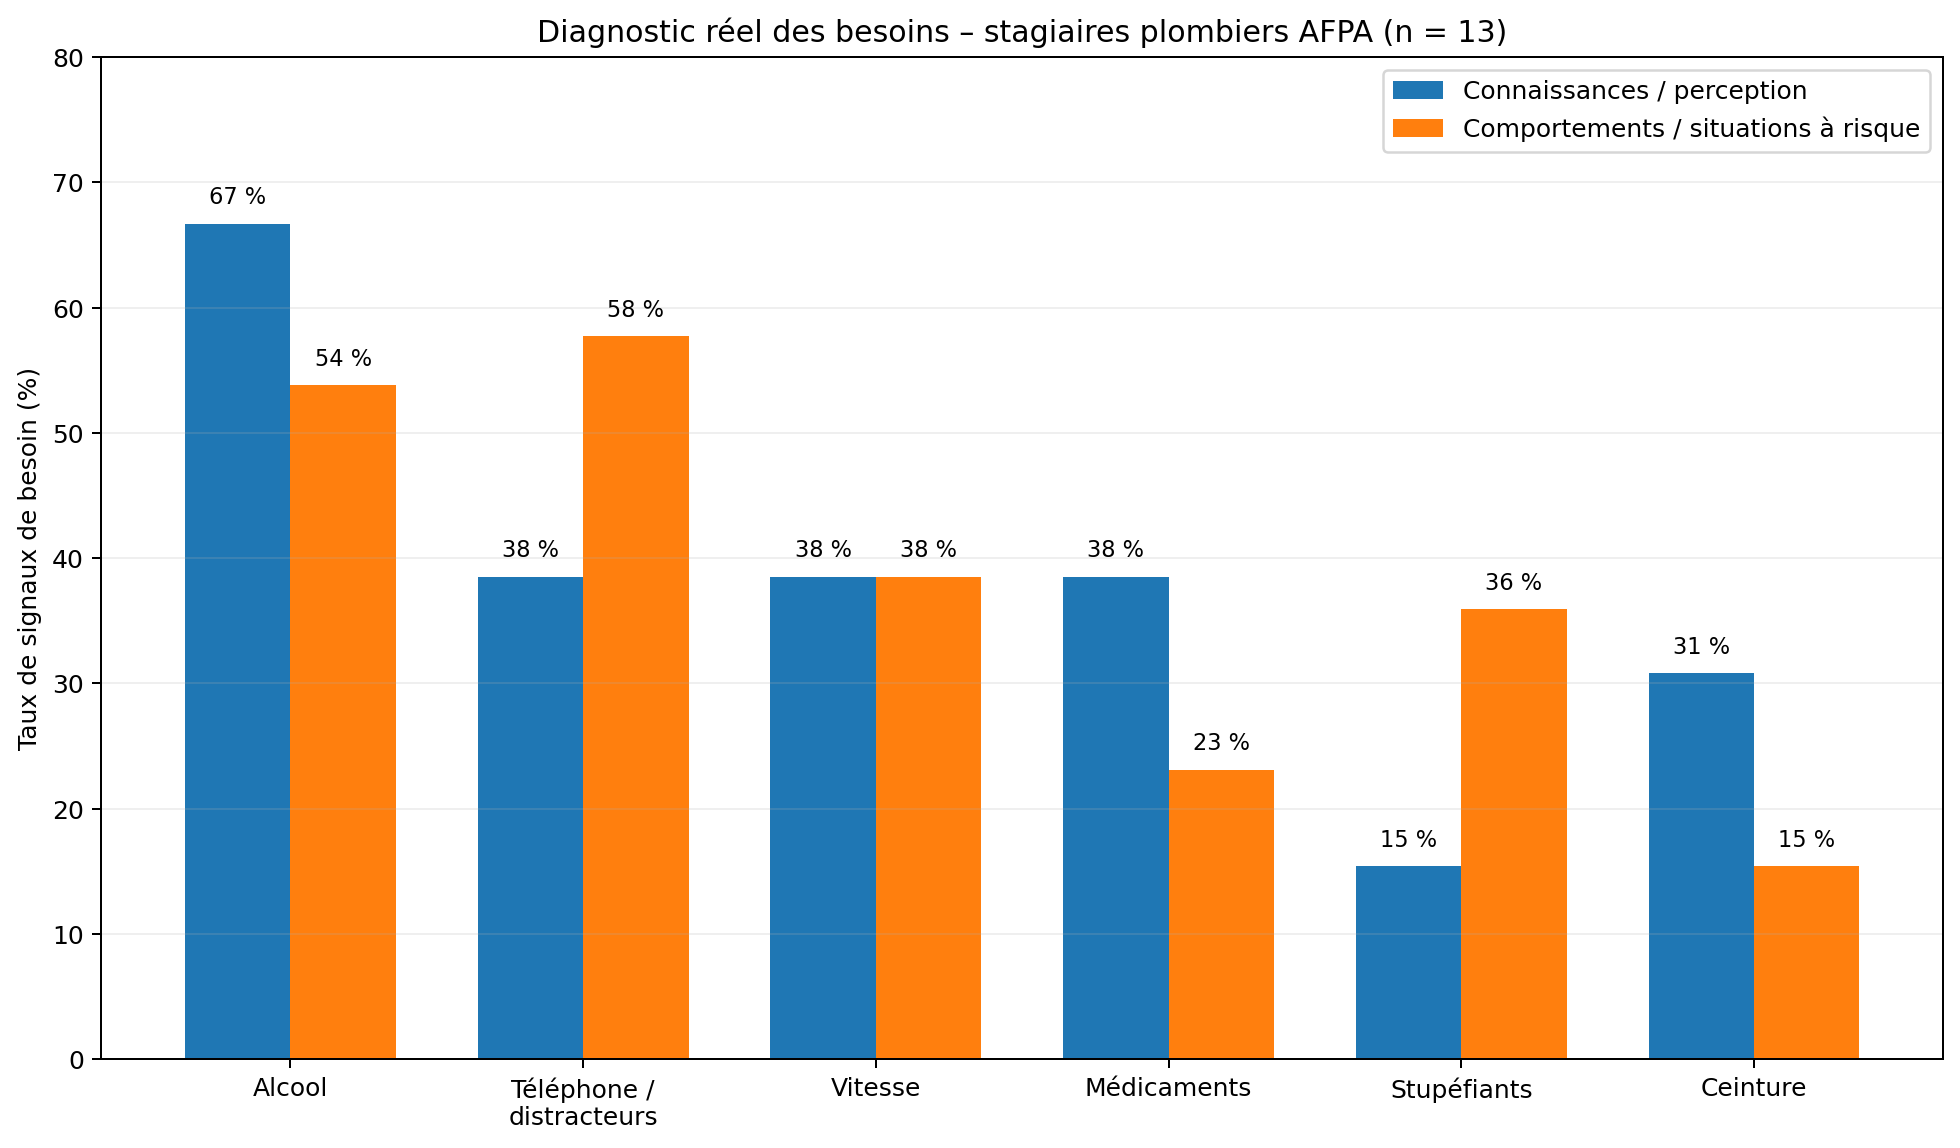
\includegraphics[width=\textwidth]{images/diagnostic_afpa_13_repondants.png}
\caption{Signaux de besoin en sécurité routière par thème, selon deux catégories d'analyse (13 répondants).}
\label{fig:diagnostic-afpa}
\end{figure}

La comparaison fait apparaître deux profils : l'alcool occupe la première place pour les connaissances et perceptions (69,23\,\%), tandis que le téléphone et les distracteurs arrivent en tête pour les comportements et situations à risque (61,54\,\%). La vitesse, les médicaments, les stupéfiants et la ceinture de sécurité présentent aussi des signaux de besoin, mais aucun ne dépasse ces deux maxima dans les catégories respectives.

\textbf{Précaution méthodologique :} la figure affiche des effectifs et des pourcentages de synthèse ; elle ne détaille pas ici les règles de construction de chaque indicateur à partir des questions du formulaire. Les valeurs sont donc présentées comme des \emph{signaux descriptifs}, et non comme le nombre de personnes ayant commis une infraction. Avec seulement treize répondants et des données déclaratives, cette analyse éclaire les choix pédagogiques pour ce groupe sans permettre de généralisation à l'ensemble de l'AFPA ou des professionnels de la plomberie. Les questions autorisant plusieurs sélections appellent la même prudence.

\section{Objectif proposé au commanditaire}
\subsection{Objectifs opérationnels du scénario « distracteurs »}
L'objectif général envisagé est d'\emph{amener les stagiaires plombiers à reconnaître les distracteurs pendant un déplacement professionnel, à expérimenter leurs effets sur l'attention et à adopter une organisation sûre face aux sollicitations}. À l'issue de la séance, chaque participant devrait pouvoir :
\begin{enumerate}[leftmargin=*]
\item citer et illustrer les quatre dimensions de la distraction : visuelle, manuelle, auditive et cognitive ;
\item expliquer, à partir d'un exemple de distance parcourue et des exercices réalisés, pourquoi quelques secondes d'inattention peuvent être dangereuses ;
\item repérer au moins deux effets d'une double tâche sur la trajectoire, le respect des consignes ou la réaction à un signal simple ;
\item identifier les risques et les pressions d'un appel ou d'un message professionnel en cours de trajet ;
\item proposer une conduite protectrice : préparer son GPS, laisser sonner, trouver un lieu de stationnement approprié, s'arrêter puis répondre.
\end{enumerate}

Ces objectifs pourront être évalués par questionnement, observation des exercices, restitution collective et quiz final. Un participant non conducteur pourra mobiliser les mêmes compétences comme futur conducteur ou usager de la route.

\section{Lettre de mission et note de cadrage}
À ce stade, les accords et les contraintes sont documentés principalement par les courriels échangés avec Mme LIÉGEOIS : intervention gratuite proposée par notre binôme, public cible de stagiaires plombiers, effectif envisagé de dix à quinze, durée d'environ deux heures et date du 4 décembre 2026 au matin. Le questionnaire commanditaire et l'entretien du 1\textsuperscript{er} octobre complètent ce cadrage.

Nous ne présentons pas ces échanges comme une lettre de mission formellement signée. Une note de cadrage reprenant les objectifs, rôles, besoins matériels, conditions d'accueil et modalités d'évaluation est proposée en annexe. Elle restera à valider avec les personnes concernées si nécessaire.

\section{Outils et méthodes utilisés}
Notre stratégie pédagogique combine la méthode interrogative, des apports courts, des supports visuels, l'observation de vidéos d'attention sélective, une démonstration comparative en extérieur et un débriefing collectif. L'objectif est de faire émerger l'écart entre \emph{se croire attentif} et \emph{disposer réellement de toutes ses ressources attentionnelles}.

Le nouveau support « Smartphone au volant : le piège des chantiers » présente le contexte professionnel, les quatre formes de distraction, des exercices d'attention sélective et de cécité attentionnelle, des ordres de grandeur de distance parcourue, la réglementation et les gestes de prévention. Sa version PDF du 13 novembre 2026 comporte trente pages ; les séquences documentées portent sur les situations de chantier, les types de distraction, deux vidéos (comptage de ballons et de passes), des données ONISR, les distances parcourues, l'article R.412-6-1, les sanctions, les réflexes préventifs et un quiz final. L'activité pédestre extérieure est une séquence complémentaire décrite dans notre protocole et dans le tableau synoptique. Le parcours pédestre « Même parcours, attention différente » prolonge ces apports par une expérience comparée sans véhicule.

La première proposition de séance « Sur la route du chantier --- Alcool et distracteurs » reste une trace de l'évolution de notre conception : elle présentait une valise dose bar, une activité SAM et différents jeux de rôle. Ces outils ne doivent pas être décrits comme réalisés ni comme nécessairement conservés dans le scénario recentré sur les distracteurs.

\subsection{Recherche de partenaires et de matériel}
La Préfecture des Alpes-Maritimes met à notre disposition une valise « dose bar », une « tête de Sam », des éthylotests, des affiches, des flyers et des goodies. Ce prêt, encadré par une convention signée, prévoit un retrait le 27 novembre 2026 et une restitution le 7 décembre 2026.

\section{Cahier des charges}
\begin{longtable}{@{}p{0.29\textwidth}p{0.64\textwidth}@{}}
\toprule
\rowcolor{bleuECSR}
\textcolor{white}{\textbf{Élément}} & \textcolor{white}{\textbf{Cadrage retenu ou point à confirmer}} \\
\midrule
\endfirsthead
\toprule
\rowcolor{bleuECSR}
\textcolor{white}{\textbf{Élément}} & \textcolor{white}{\textbf{Cadrage retenu ou point à confirmer}} \\ \midrule
\endhead
Commanditaire & AFPA Nice, interlocutrice : Mme Muriel LIÉGEOIS. \\
Intervenants & Sam FOKAM WABO et Manane SADIK, stagiaires TP ECSR, en co-animation. \\
Public & Promotion de stagiaires plombiers ; treize répondants au diagnostic ; effectif du jour à relever. \\
Date et horaire & 4 décembre 2026 au matin ; horaire exact à confirmer. \\
Durée & Environ deux heures, à répartir entre accueil, apports, activités et bilan. \\
Lieu & AFPA Nice ; salle de formation et parcours pédestre extérieur, sous réserve d’autorisation et de reconnaissance préalable du terrain. \\
Objectif général & Reconnaître les distracteurs et décider comment gérer sans risque les sollicitations professionnelles ; scénario récent à confirmer avec le commanditaire. \\
Méthodes & Interrogative, participative, visionnage guidé, expérimentation pédestre, observation comparée et débriefing. \\
Moyens & Vidéoprojecteur, tableau, supports de séance et matériels de prévention ; inventaire final à confirmer ; convention signée par la directrice de cabinet transmise le 10 novembre, retrait prévu le 27 novembre et restitution le 7 décembre au matin. \\
Sécurité & Aucun véhicule en mouvement ni consommation d’alcool ; parcours exclusivement à pied, aire isolée et dégagée, consignes de non-collision, balle souple sans visée du visage, possibilité de refuser une tâche. \\
Évaluation & Questions de vérification, mises en situation, questionnaire de satisfaction et retour commanditaire à recueillir. \\
Traçabilité & Questionnaires anonymisés, échanges, convention, supports, tableau synoptique et bilan de séance. \\
\bottomrule
\end{longtable}

\section{Tableau synoptique}
Le tableau synoptique ci-après reprend les \textbf{six colonnes du modèle fourni} : séquences, objectif, durée, contenu, méthodes/techniques et moyen. Afin de conserver ces rubriques sans réduire excessivement la lisibilité, \textbf{seule la page du tableau} est présentée au format paysage. Il s'agit d'une \emph{préparation} de deux heures, susceptible d'être ajustée selon les conditions de l'intervention du 4 décembre 2026.

\clearpage
\newgeometry{left=0.8cm,right=0.8cm,top=1.2cm,bottom=1.2cm}
\begin{landscape}
\thispagestyle{plain}
\begin{center}
{\Large\bfseries Tableau synoptique prévisionnel -- Sensibilisation aux distracteurs}\\[2pt]
{\small AFPA Nice -- stagiaires plombiers -- co-animation -- durée totale : 120 minutes}
\end{center}
\vspace{1mm}
\begingroup
\scriptsize
\setlength{\arrayrulewidth}{0.4pt}
\renewcommand{\arraystretch}{1.05}
\setlength{\tabcolsep}{2pt}
%\begin{adjustbox}{max totalsize={\linewidth}{0.90\textheight},center}
\begin{adjustbox}{width=\linewidth,center}
%\begin{tabular}{@{}p{2.9cm}p{4.0cm}p{1.4cm}p{6.0cm}p{4.1cm}p{3.8cm}@{}}
\begin{tabular}{@{}p{3.2cm}p{4.4cm}p{1.5cm}p{6.8cm}p{4.6cm}p{4.3cm}@{}}
%\begin{tabular}{|p{3.2cm}|p{4.4cm}|p{1.5cm}|p{6.8cm}|p{4.6cm}|p{4.3cm}|}
\toprule
\rowcolor{bleuECSR}
\textcolor{white}{\textbf{Séquences}} & \textcolor{white}{\textbf{Objectif}} & \textcolor{white}{\textbf{Durée}} & \textcolor{white}{\textbf{Contenu}} & \textcolor{white}{\textbf{Méthodes/Techniques}} & \textcolor{white}{\textbf{Moyen}} \\
\midrule
% Coloration explicite de chaque ligne : stable avec booktabs et adjustbox.
\rowcolor{orangeECSR!18}
Présentation / accueil & Identifier les attentes et installer un climat de confiance. & 8 min & Présentation des intervenants ; métier de plombier, déplacements et attentes des participants. & Tour de table bref ; questionnement oral. & Diaporama, vidéoprojecteur, tableau. \\
\midrule
Question d'ouverture & Susciter l'intérêt et faire émerger la problématique. & 2 min & « Un appel client urgent justifie-t-il de répondre immédiatement au volant ? » & Question d'accroche ; débat flash. & Diapositive, tableau. \\
\midrule
\rowcolor{orangeECSR!18}
Évaluation initiale & Repérer les représentations et connaissances de départ. & 6 min & Reconnaissance des distracteurs ; risques du mains-libres ; réaction à un SMS professionnel. & Questions diagnostiques ; vote / échanges ; sans jugement. & Questions projetées, tableau, feutres. \\
\midrule
Annonce des objectifs & Faire comprendre les acquis recherchés. & 4 min & Identifier les distractions ; observer l'effet de la double tâche ; choisir une réponse sûre face aux sollicitations. & Présentation interrogative ; reformulation. & Diaporama, tableau. \\
\midrule
\rowcolor{orangeECSR!18}
Cours : types de distraction & Distinguer les quatre formes de distraction. & 13 min & Distractions visuelle, manuelle, auditive et cognitive ; exemples d'appel, SMS, GPS, recherche d'adresse. & Exposé dialogué ; exemples métier. & Diaporama, vidéoprojecteur. \\
\midrule
Mise en évidence de l'attention & Constater les limites de l'attention sélective. & 12 min & Vidéo(s) d'observation ; repérage d'éléments inattendus ; comparaison des perceptions. & Observation individuelle ; débat / débriefing. & Vidéo préchargée, ordinateur, écran ; variante orale. \\
\midrule
\rowcolor{orangeECSR!18}
Cours : risques et règles & Relier la distraction aux conséquences routières et au droit. & 15 min & Distance parcourue sans regarder la route ; risque de collision ; interdictions et sanctions du téléphone tenu en main. & Exposé interactif ; calcul simple ; questions. & Diaporama, tableau, sources réglementaires. \\
\midrule
Réflexes professionnels & Savoir gérer un appel ou message pendant un trajet. & 8 min & Anticiper les communications ; laisser sonner ; stationner dans un lieu sûr ; rappeler à l'arrêt. & Étude de cas « client / chef de chantier » ; échange. & Diaporama, fiche scénario. \\
\midrule
\rowcolor{orangeECSR!18}
Préparation extérieure & Connaître les consignes et les critères d'observation. & 8 min & Présentation du parcours pédestre ; volontaires, observateurs, sécurité ; temps, erreurs, hésitations. & Démonstration ; répartition des rôles. & 4--5 plots, objets, téléphone factice, fiches, chronomètre. \\
\midrule
Opérationnalisation : parcours & Expérimenter la double tâche et observer ses effets. & 32 min & Même parcours sans distracteur, puis appel, SMS, événement visuel avec balle souple, sollicitations cumulées (si réalisable). & Expérimentation à pied ; observation comparée ; rotations ciblées de volontaires. & Plots, téléphone, SMS préparés, balle en mousse, chronomètre, grille. \\
\midrule
\rowcolor{orangeECSR!18}
Débriefing / transfert & Identifier les écarts et transposer à la conduite d'un utilitaire. & 8 min & Comparaison des temps, erreurs et réactions ; place des pressions professionnelles ; stratégies de prévention. & Analyse collective ; mise en commun des observations. & Grille d'observation, tableau, feutres. \\
\midrule
Bilan final / évaluation & Vérifier les acquis et fixer une conduite à tenir. & 4 min & Questions de contrôle ; reformulation du réflexe « s'arrêter avant de répondre » ; conclusion et remerciements. & Évaluation orale flash ; synthèse. & Questions de bilan, tableau. \\
\midrule
\rowcolor{bleuECSR}\textcolor{white}{\textbf{TOTAL}} & \textcolor{white}{\textbf{Séance prévisionnelle (intérieur et extérieur).}} & \textcolor{white}{\textbf{120 min}} & \multicolumn{3}{>{\columncolor{bleuECSR}}l}{\textcolor{white}{\textit{Temps indicatifs, à ajuster après observation de l\'action réelle.}}} \\
\bottomrule
\end{tabular}
\end{adjustbox}
\endgroup
\end{landscape}
\restoregeometry
\clearpage

\paragraph{Contraintes de faisabilité.}
Quinze stagiaires sont envisagés, mais il ne serait pas réaliste de leur faire réaliser individuellement les cinq passages dans une enveloppe de 35 minutes. L'atelier repose donc sur \textbf{quelques volontaires avec observation active du reste du groupe} : les observateurs notent les indicateurs, comparent les essais et participent au débriefing. Les passages sont adaptables selon l'effectif présent et les conditions matérielles. Aucun résultat ne sera annoncé d'avance : le chronométrage et les erreurs seront relevés sur place.

\paragraph{Vigilance documentaire.}
Le diaporama contient des chiffres d'accidentalité, des pourcentages et des sanctions qui devront être contrôlés dans leurs sources officielles et situés à leur bonne date avant l'animation. Les vidéos ne peuvent être utilisées que si leur diffusion est autorisée et si le matériel de projection fonctionne ; une variante orale de l'exercice devra être prévue.

\chapter{Contenu de la réponse}

\noindent\fcolorbox{orangeECSR}{orangeECSR!7}{\parbox{0.94\textwidth}{\textbf{Statut de ce chapitre : récit rédigé à titre provisoire avant l'action.} Les verbes au passé sont une mise en forme anticipée, demandée pour préparer la version finale du mémoire ; ils ne constituent pas une attestation de réalisation. Après le 4 décembre 2026, les horaires, activités, réactions, observations et évaluations devront être confrontés aux faits et corrigés.}}

\section{Contenu et déroulement de l'action}
\subsection{Accueil, présentation et ancrage dans le métier de plombier}
Nous avons introduit notre séance par le titre de notre support : \og Smartphone au volant : le piège des chantiers \fg{}. Notre intention était de placer les stagiaires dans une situation professionnelle concrète et de montrer que le risque routier ne concerne pas uniquement le trajet domicile--formation : il peut aussi survenir lors des déplacements entre une entreprise, un fournisseur, un client et un chantier.

Après la présentation de notre binôme et le rappel du cadre de cette sensibilisation, nous avons évoqué quatre situations familières ou plausibles dans le métier : l'appel urgent d'un client, la recherche d'une adresse sur le GPS, le retard pris sur un chantier et l'envoi d'une photographie à un responsable. Nous avons posé une question d'accroche : \og Lorsqu'un client vous appelle pour une urgence alors que vous conduisez, devez-vous répondre immédiatement ? \fg{} Cette question devait susciter les premières réactions, sans jugement et sans chercher d'emblée une réponse unique.

Nous avons ensuite annoncé les quatre objectifs affichés dans le diaporama : identifier les risques liés au téléphone et aux distracteurs ; comprendre leurs conséquences sur la conduite ; connaître les règles et sanctions ; adopter des réflexes sûrs pour l'activité professionnelle. Nous avons souligné que la perte d'attention peut avoir des conséquences humaines et matérielles, mais aussi compromettre l'exercice d'un métier nécessitant des déplacements. \emph{La formulation du support selon laquelle la perte du permis entraînerait systématiquement la perte de l'employabilité a été traitée comme un message de vigilance, et non comme une règle applicable à toute situation individuelle.}

\subsection{Identifier les quatre dimensions de la distraction}
Nous avons organisé un apport dialogué autour des quatre dimensions de la distraction présentées dans les diapositives 8 à 12 :
\begin{description}[leftmargin=3.0cm,style=nextline]
\item[Visuelle] Détourner le regard de l'environnement routier, par exemple pour consulter un message, une notification ou l'écran du GPS.
\item[Manuelle] Mobiliser une main pour composer un numéro, manipuler un téléphone ou régler un équipement au lieu de garder les gestes nécessaires à la conduite.
\item[Auditive] Voir son attention sollicitée par une sonnerie, une conversation ou un signal sonore, notamment dans une situation d'urgence professionnelle.
\item[Cognitive] Consacrer ses ressources mentales à un échange stressant, à un problème de chantier ou à l'organisation de la prochaine intervention plutôt qu'à l'analyse de la circulation.
\end{description}
Nous avons insisté sur le fait qu'une même situation pouvait cumuler plusieurs dimensions : lire un SMS associe, notamment, distraction visuelle, manuelle et cognitive. Le cas du téléphone en mains libres a servi à distinguer la conformité de certains dispositifs avec la réglementation de l'absence de risque : une conversation peut encore mobiliser l'attention du conducteur.

\subsection{Deux activités vidéo sur les limites de l'attention}
Pour rendre les notions moins abstraites, nous avons utilisé deux exercices d'observation figurant dans notre support. Le premier consistait à compter des ballons selon une consigne donnée ; le second demandait de compter des passes dans une vidéo. Les participants devaient conserver leur réponse jusqu'à la fin du visionnage, puis discuter de ce qu'ils avaient vu et de ce qui pouvait leur avoir échappé.

Notre objectif n'était pas de mesurer médicalement l'attention des stagiaires, mais de faire comprendre qu'une tâche ciblée peut mobiliser fortement les ressources cognitives et réduire la perception d'autres événements. Nous avons relié ce phénomène au fait de rechercher une adresse, de répondre à un client ou de consulter un écran pendant la conduite. Les vidéos étaient des supports de discussion ; leurs résultats individuels ne devaient pas donner lieu à un classement des participants.

\subsection{Chiffres, distance parcourue et conséquences professionnelles}
Nous avons poursuivi par un éclairage sur la sécurité routière, à partir des diapositives consacrées aux données de l'ONISR et aux risques des distracteurs. Le support présentait notamment des chiffres de mortalité et de blessés en 2025, ainsi que des données de 2024 concernant le défaut d'attention et l'usage du téléphone chez les conducteurs de véhicules utilitaires. Nous avons présenté ces données comme des éléments de contextualisation et non comme des résultats issus du groupe de stagiaires. \emph{Les valeurs précises, leurs définitions et leurs sources devront être revérifiées dans la version définitive remise au jury.}

Nous avons ensuite proposé un calcul simple pour illustrer l'effet d'un regard détourné pendant cinq secondes. À vitesse constante, la distance parcourue est égale à la vitesse exprimée en mètres par seconde multipliée par le temps. Nous avons présenté les ordres de grandeur figurant dans le support : environ 70 mètres à 50 km/h, 110 mètres à 80 km/h, 125 mètres à 90 km/h et 180 mètres à 130 km/h. La discussion ne visait pas à prétendre qu'un conducteur ne perçoit nécessairement rien pendant cinq secondes ; elle montrait qu'un véhicule continue de se déplacer pendant que son conducteur réduit sa prise d'informations.

Les exemples d'un piéton traversant, d'un véhicule freinant ou d'une intervention sur chaussée ont permis de faire le lien avec les risques concrets. Nous avons rapproché ces situations de la pression professionnelle : désir de satisfaire le client, retard sur le planning, consignes du responsable ou urgence apparente.

\subsection{Cadre réglementaire et réflexes de prévention}
Nous avons consacré une séquence aux règles applicables à l'usage du téléphone au volant, en prenant pour référence l'article R.412-6-1 du Code de la route. Le support rappelait notamment l'interdiction de tenir un téléphone en main et celle de porter à l'oreille certains dispositifs émettant du son, sous réserve des exceptions réglementaires. Les sanctions mises en avant étaient une amende forfaitaire de 135 euros et le retrait de trois points pour l'infraction correspondante ; des conséquences supplémentaires peuvent exister dans certaines situations prévues par les textes. Nous avons distingué la sanction juridique du risque d'accident, qui demeure l'enjeu central de la sensibilisation.

Nous avons terminé cette partie par la recherche de mesures préventives applicables au métier : programmer son GPS avant de partir, activer si possible le mode conduite, placer le téléphone hors de portée, prévenir les clients de son indisponibilité temporaire, et s'arrêter sur un emplacement autorisé et sécurisé avant de rappeler ou de consulter un message. Nous avons insisté sur le rôle de l'organisation du travail : un appel considéré comme urgent ne doit pas imposer au conducteur de traiter une sollicitation en mouvement.

\subsection{Activité extérieure : « Même parcours, attention différente »}
Pour prolonger les apports théoriques, nous avons organisé une expérimentation exclusivement \textbf{pédestre}, sur un parcours balisé de huit à douze mètres. Ce parcours comportait quatre ou cinq plots à contourner, une zone d'arrêt, un objet à toucher ou récupérer, puis une ligne d'arrivée. La configuration permettait de reproduire une tâche simple, sans circulation de véhicule et sans recherche de vitesse.

L'effectif de référence étant de quinze stagiaires, nous avons retenu des passages par volontaires, les autres participants occupant un rôle d'observateur. Nous avons expliqué les critères d'observation : durée du parcours, plots touchés, sorties du tracé, hésitations, oublis de consigne, durée de regard détourné et réaction à un événement visuel. Nous avons précisé que les mesures n'avaient aucune valeur de diagnostic individuel et qu'elles servaient uniquement au débat pédagogique.

\paragraph{Premier passage : parcours de référence sans distracteur.}
Un volontaire a reçu la consigne de réaliser normalement le slalom, de s'arrêter à l'endroit indiqué, de toucher l'objet prévu et de franchir la ligne d'arrivée. Le temps et les éventuelles erreurs ont servi de référence pour comparer les conditions suivantes. Nous avons commencé le débriefing par une question ouverte sur la difficulté ressentie.

\paragraph{Deuxième passage : appel professionnel.}
Le même parcours a été repris avec la simulation d'un appel imprévu, préparé par un animateur : \og Bonjour, c'est urgent. Le client attend. Pouvez-vous me confirmer l'adresse du prochain chantier ? \fg{} Les observateurs devaient relever si le participant s'arrêtait, cherchait à décrocher, ralentissait, oubliait une étape ou touchait un plot. Nous avons interrogé le groupe sur ce qui aurait pu se passer si l'événement s'était produit au volant d'un utilitaire.

\paragraph{Troisième passage : lecture d'un SMS.}
Nous avons introduit un message bref de type professionnel : \og Nouveau chantier : 12 rue des Lilas. Le client attend depuis 20 minutes. \fg{} Le volontaire devait lire l'information et la restituer, sans accélérer et avec la possibilité de s'arrêter immédiatement. L'observation portait sur le regard détourné, la trajectoire, les hésitations et les consignes oubliées. Nous avons relié cet essai au cumul des dimensions visuelle, manuelle et cognitive.

\paragraph{Quatrième passage : double tâche et événement visuel.}
Le parcours a été associé à une information à écouter ou à lire ainsi qu'à un signal visuel simple : une balle en mousse présentée ou envoyée très doucement, sans viser la tête. Les volontaires étaient prévenus de la possibilité de cet événement, mais pas de son instant exact. Attraper la balle restait facultatif ; il était interdit de courir ou de se jeter pour l'atteindre. L'objectif était d'observer la disponibilité attentionnelle, sans mettre les stagiaires en situation de chute.

\paragraph{Cinquième passage : sollicitations cumulées, si les conditions le permettaient.}
Un dernier essai facultatif associait lecture d'une information, question orale et événement visuel. Nous avons utilisé ce cas comme analogie des situations professionnelles dans lesquelles le GPS, le client, le responsable et le retard sollicitent simultanément le conducteur. \emph{Le maintien de ce passage dans le récit définitif dépendra de sa réalisation effective le jour de l'action.}

\paragraph{Débriefing et transfert professionnel.}
Nous avons organisé la mise en commun des observations en distinguant les différents passages, sans présumer d'une augmentation systématique des temps ou des erreurs. Quatre questions ont structuré les échanges : qu'est-ce qui a changé ? Aviez-vous conscience des difficultés éventuelles ? Quelle sollicitation vous a le plus perturbés ? Quelle décision adopter avant de répondre à un appel ou à un message au volant ?

La comparaison était volontairement présentée comme une \textbf{analogie pédagogique} : toucher un plot dans un environnement sécurisé n'a pas la gravité d'une collision avec un piéton ou un cycliste. Un parcours à pied ne permet pas de quantifier le risque d'accident en voiture ; il aide à prendre conscience de la concurrence entre les tâches et à discuter des décisions protectrices.

\subsection{Organisation de la co-animation et sécurité}
Nous avons préparé une répartition fonctionnelle des responsabilités : un intervenant présentait les consignes et conduisait le questionnement, tandis que l'autre gérait le matériel, le temps et la sécurisation du passage. Les rôles pouvaient être inversés lors des séquences. La zone extérieure devait être dégagée, isolée de toute circulation et exempte d'obstacles dangereux. Les déplacements se faisaient uniquement en marchant. Les messages étaient fictifs, les observations anonymes et chacun pouvait refuser une sollicitation ou interrompre l'exercice.

La transition entre la salle et l'extérieur, ainsi que le retour collectif, avaient été pris en compte dans le minutage du tableau synoptique de deux heures. Quelques volontaires réalisaient les essais successifs pendant que les autres notaient des observations ; nous ne prévoyions pas cinq passages pour chacun des quinze stagiaires.

\section{Évaluation des acquis à chaud}
Nous avons terminé le scénario par un quiz oral inspiré de la diapositive « Testez vos connaissances ». Quatre questions portaient sur les types de distraction, la sanction du téléphone en main, la distance parcourue en cinq secondes à 90 km/h et l'importance du défaut d'attention dans les accidents. Nous avons également prévu une question d'application : \og Un client appelle alors que vous êtes au volant pour vous annoncer une urgence : que faites-vous ? \fg{}

L'évaluation devait vérifier non seulement la mémorisation d'une donnée, mais surtout la capacité à proposer une réponse sûre : ne pas traiter la sollicitation pendant la conduite, rechercher un lieu autorisé où stationner et rappeler à l'arrêt. Les réponses des observateurs au parcours étaient considérées au même titre que celles des volontaires. Aucune note individuelle n'était recherchée.

\textbf{Données à reporter après l'action :} nombre de participants présents et évalués, questions réellement posées, répartition des réponses, erreurs fréquentes et éventuelles reformulations. Aucune progression mesurée ni réussite collective n'est affirmée à ce stade.

\section{Questionnaire de satisfaction}
Nous avons préparé un questionnaire anonyme distinct du quiz, portant sur la clarté des explications, l'intérêt des deux vidéos, l'utilité du parcours pédestre, la pertinence des situations de chantier, le temps laissé aux échanges et les comportements que les participants envisagent de modifier. Une question ouverte permettait de proposer des améliorations.

\textbf{Données à reporter après l'action :} questionnaire effectivement administré, nombre de retours, synthèse des appréciations et propositions recueillies. Les intentions exprimées ne seront pas assimilées à un changement durable du comportement routier.

\section{Vérification du compte rendu après l'intervention}
\texteguide{Au retour du 4 décembre : vérifier le contenu réellement projeté (y compris la lecture effective des vidéos), les durées et l'effectif ; supprimer tout passage non réalisé ; renseigner les rôles effectifs du binôme, les observations du parcours, les résultats du quiz et la satisfaction ; remplacer le présent encadré provisoire par un compte rendu exclusivement factuel.}

\begingroup\color{red}
\chapter{Analyse de la prestation}
Ce chapitre sera finalisé après l’action. Je préfère ne pas écrire à l’avance des points forts ou des difficultés qui n’ont pas encore été observés.

\section{Ce qui a fonctionné et ce qui a moins bien fonctionné}

Après la séance, je m’appuierai sur des faits précis : participation du groupe, compréhension des consignes, gestion du temps, qualité des échanges, fonctionnement du binôme et sécurité de l’activité extérieure.

[À compléter : Présenter deux ou trois faits précis observés le 4 décembre. Pour chacun : ce qui s’est passé, pourquoi cela a pu se produire, quel effet cela a eu sur la séance et ce que j’en retiens.]

\section{Retours des stagiaires et du commanditaire}

Je comparerai les résultats du quiz, les réponses au questionnaire de satisfaction et le retour de Mme LIÉGEOIS avec les attentes identifiées au début du projet.

[À compléter : Ajouter le nombre de réponses recueillies, les tendances principales, quelques remarques anonymisées si elles sont utiles, et le retour du commanditaire.]

\section{Ce que je changerais}

L’objectif de cette partie sera de montrer ce que j’ai appris comme futur ECSR. Les améliorations devront être directement liées aux constats : simplifier une consigne, modifier une durée, mieux intégrer les non-conducteurs, ajuster le support ou approfondir un débriefing.

[À compléter : Rédiger des améliorations concrètes et réalistes : ce que je garderais, ce que je modifierais et ce que je ferais différemment lors d’une prochaine action.]
\endgroup

\chapter{Veille réglementaire et documentaire}
\section{Ma méthode de vérification}

Pour préparer la séance, je dois distinguer les règles juridiques, les statistiques d’accidentalité et les recommandations de prévention. Je privilégie donc les sources institutionnelles et je vérifie la date des informations avant de les utiliser dans le diaporama.

Mes principales sources sont :

— Légifrance et le Code de la route pour les textes applicables, notamment l’article R.412-6-1

sur le téléphone ;

— l’ONISR pour les bilans d’accidentalité et les observations de comportements ;

— Sécurité routière et Service-Public.fr pour les informations accessibles sur les règles et

les sanctions ;

— l’INRS, la CNAM et la MSA pour le risque routier professionnel et l’organisation des

déplacements en mission.

Cette veille a une utilité directe : elle me permet de corriger ou d’actualiser une donnée avant de la présenter. Elle m’aide aussi à choisir des informations utiles au public plutôt qu’à multiplier les chiffres.

Par exemple, pour les distracteurs, je dois faire attention aux termes utilisés. L’inattention, l’usage du téléphone et les distracteurs technologiques ne sont pas toujours regroupés de la même manière dans les statistiques. Je dois donc présenter chaque chiffre avec son année et son périmètre, sans lui faire dire plus que la source. De la même façon, les données concernant les véhicules utilitaires ne doivent pas être présentées comme si tous les accidents étaient liés au téléphone.

Cette rigueur fait partie de ma posture de futur ECSR. Si une information évolue entre la préparation du document écrit et la date de l’animation, c’est la donnée la plus récente et la mieux sourcée qui doit être utilisée.

[À compléter : Avant la remise définitive : ajouter un tableau court avec les documents réellement consultés, leur date, le point vérifié et l’incidence sur la séance.]

\chapter{Conclusion de l'action}

\section{Bilan général}
La phase préparatoire nous a permis de construire une proposition fondée sur une démarche de diagnostic plutôt que sur un thème imposé. Après la prise de contact avec l'AFPA, nous avons complété les attentes du commanditaire par un questionnaire destiné aux stagiaires. L'analyse de treize réponses fait apparaître des lacunes importantes concernant l'alcool, ainsi que des comportements déclarés préoccupants liés au téléphone et aux distracteurs.

Cette préparation a également nécessité d'anticiper les conditions d'animation, de rechercher des ressources auprès de la Préfecture et de concevoir des situations adaptées aux déplacements du métier de plombier. À ce stade, ces acquis concernent la \emph{préparation} de l'action et non les résultats d'une sensibilisation déjà conduite.

\texteguide{Après l'intervention : compléter la conclusion avec le bilan réel, l'atteinte des objectifs, les limites du dispositif, les enseignements personnels en tant que futur ECSR et les perspectives de remédiation.}

\chapter{Remerciements}
Je tiens à remercier les personnes et les structures qui m’ont accompagné dans ma formation et dans la préparation de cette action de sensibilisation. L’AFPA de Nice et Mme Muriel LIÉGEOIS : pour leur confiance, leur accueil et leur collaboration dans l’identification des besoins des stagiaires. La Préfecture des Alpes-Maritimes, Mme Nadia HULIN et Mme Anaïs CANDAT : pour leur disponibilité et leur accompagnement dans la recherche et l’organisation du prêt de matériel pédagogique. France Travail : pour son accompagnement dans mon projet de reconversion professionnelle. L’AFTRAL et ses formateurs : pour la qualité de leur accompagnement, leurs conseils et les compétences pédagogiques transmises. Les auto-écoles qui m’ont accueilli en stage, en particulier l’équipe de l’auto-école Saint Barthelemy : pour leur accueil et les expériences professionnelles qui ont enrichi mon apprentissage du métier d’ECSR. Ma collègue Manane SADIK : pour son engagement, sa coopération et le travail mené ensemble tout au long de ce projet. Mon groupe de formation : pour l’entraide, les échanges et le partage d’expériences qui ont nourri ma progression. Ma famille : pour sa patience, sa compréhension et son soutien constant pendant cette formation.

\appendix
\chapter{Annexes}

\section{Inventaire des pièces justificatives}
Les annexes sont destinées à fournir des preuves utiles, sans reproduire l'intégralité de la correspondance ni divulguer inutilement des coordonnées personnelles. Les noms des interlocuteurs institutionnels sont conservés dans le corps du mémoire lorsqu'ils sont nécessaires à la compréhension de la démarche ; les adresses privées, numéros de téléphone et identifiants sont à masquer sur toute copie diffusée.

\begin{longtable}{@{}p{0.13\textwidth}p{0.57\textwidth}p{0.20\textwidth}@{}}
\toprule
\rowcolor{bleuECSR}
\textcolor{white}{\textbf{Repère}} & \textcolor{white}{\textbf{Pièce à classer}} & \textcolor{white}{\textbf{Situation}} \\
\midrule
\endfirsthead
\toprule
\rowcolor{bleuECSR}
\textcolor{white}{\textbf{Repère}} & \textcolor{white}{\textbf{Pièce à classer}} & \textcolor{white}{\textbf{Situation}} \\ \midrule
\endhead
A1 & Courriel de proposition du 9 septembre 2026 et réponse favorable du 10 septembre. & Disponible \\
A2 & Questionnaire de recueil des besoins commanditaire et réponse transmise le 29 septembre. & Disponible \\
A3 & Courriels des 28--29 septembre : demande d'entretien, correction de date et confirmation du rendez-vous du 1\textsuperscript{er} octobre. & Disponible \\
A4 & Questionnaire anonyme de 30 questions adressé aux stagiaires le 26 octobre. & Disponible \\
A5 & Courriels du 26 et du 29 octobre relatifs à la diffusion, la relance et la transmission annoncée des réponses. & Disponible \\
A6 & Synthèse agrégée des treize réponses et graphique comparatif des besoins. & Disponible \\
A7 & Demande de matériel du 11 octobre et réponse du Bureau de la sécurité routière du 12 octobre. & Disponible \\
A8 & Convention de prêt envoyée le 30 octobre ; convention contresignée et transmise le 10 novembre ; échanges des 10--12 novembre sur les dates et horaires de retrait et restitution et demande d'accès au CADAM. & Échanges disponibles ; exécution à confirmer \\
A9 & Diaporama initial « Sur la route du chantier --- Alcool et distracteurs » et support de 30 pages « Smartphone au volant : le piège des chantiers » (version du 13 novembre 2026). & Disponibles \\
A10 & Tableau synoptique prévisionnel de deux heures ; protocole extérieur « Même parcours, attention différente » et grille vierge d’observation. & Rédigés ; à valider \\
A11 & Grille d'évaluation des acquis et questionnaire de satisfaction utilisés. & À finaliser \\
A12 & Bilan de l'action, retour commanditaire et autoanalyse. & Après le 4 déc. \\
\bottomrule
\end{longtable}



\section{Échanges avec le commanditaire : premier contact (A1)}
Courriels qui documentent la proposition initiale et la transmission du premier questionnaire.

\clearpage
\begin{landscape}
\thispagestyle{plain}
\noindent{\large\bfseries 9 septembre 2026 — Proposition initiale de sensibilisation}\par\medskip
\begin{center}

\includegraphics[width=0.97\linewidth,height=0.77\textheight,keepaspectratio]{images/annexes/echanges/a01_20260909_proposition.png}
\end{center}
\end{landscape}

\clearpage
\begin{landscape}
\thispagestyle{plain}
\noindent{\large\bfseries 10 septembre — Réponse favorable de Mme Liégeois}\par\medskip
\begin{center}

\includegraphics[width=0.97\linewidth,height=0.77\textheight,keepaspectratio]{images/annexes/echanges/a02_20260910_accord.png}
\end{center}
\end{landscape}

\clearpage
\begin{landscape}
\thispagestyle{plain}
\noindent{\large\bfseries 11 septembre — Premier envoi annoncé du questionnaire}\par\medskip
\begin{center}

\includegraphics[width=0.97\linewidth,height=0.77\textheight,keepaspectratio]{images/annexes/echanges/a03_20260911_envoi_quest.png}
\end{center}
\end{landscape}

\clearpage
\begin{landscape}
\thispagestyle{plain}
\noindent{\large\bfseries 11 septembre — Signalement de la pièce jointe manquante}\par\medskip
\begin{center}
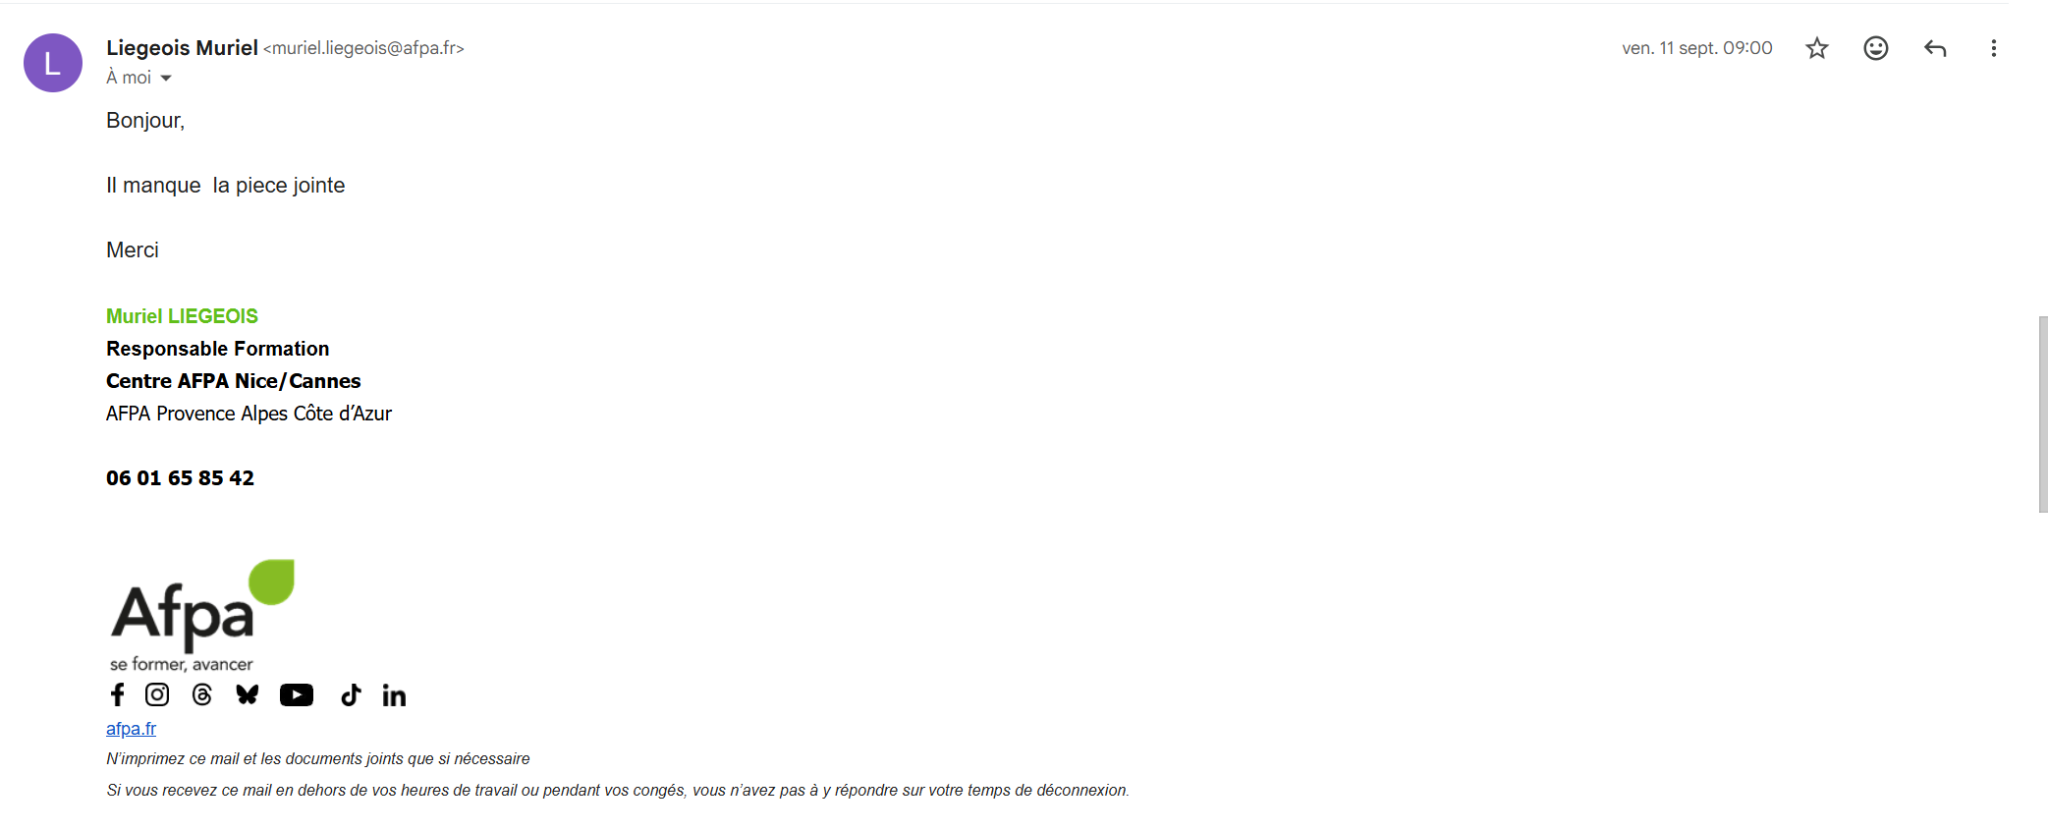
\includegraphics[width=0.97\linewidth,height=0.77\textheight,keepaspectratio]{images/annexes/echanges/a04_20260911_pj_absente.png}
\end{center}
\end{landscape}

\clearpage
\begin{landscape}
\thispagestyle{plain}
\noindent{\large\bfseries 23 septembre — Transmission effective du questionnaire}\par\medskip
\begin{center}
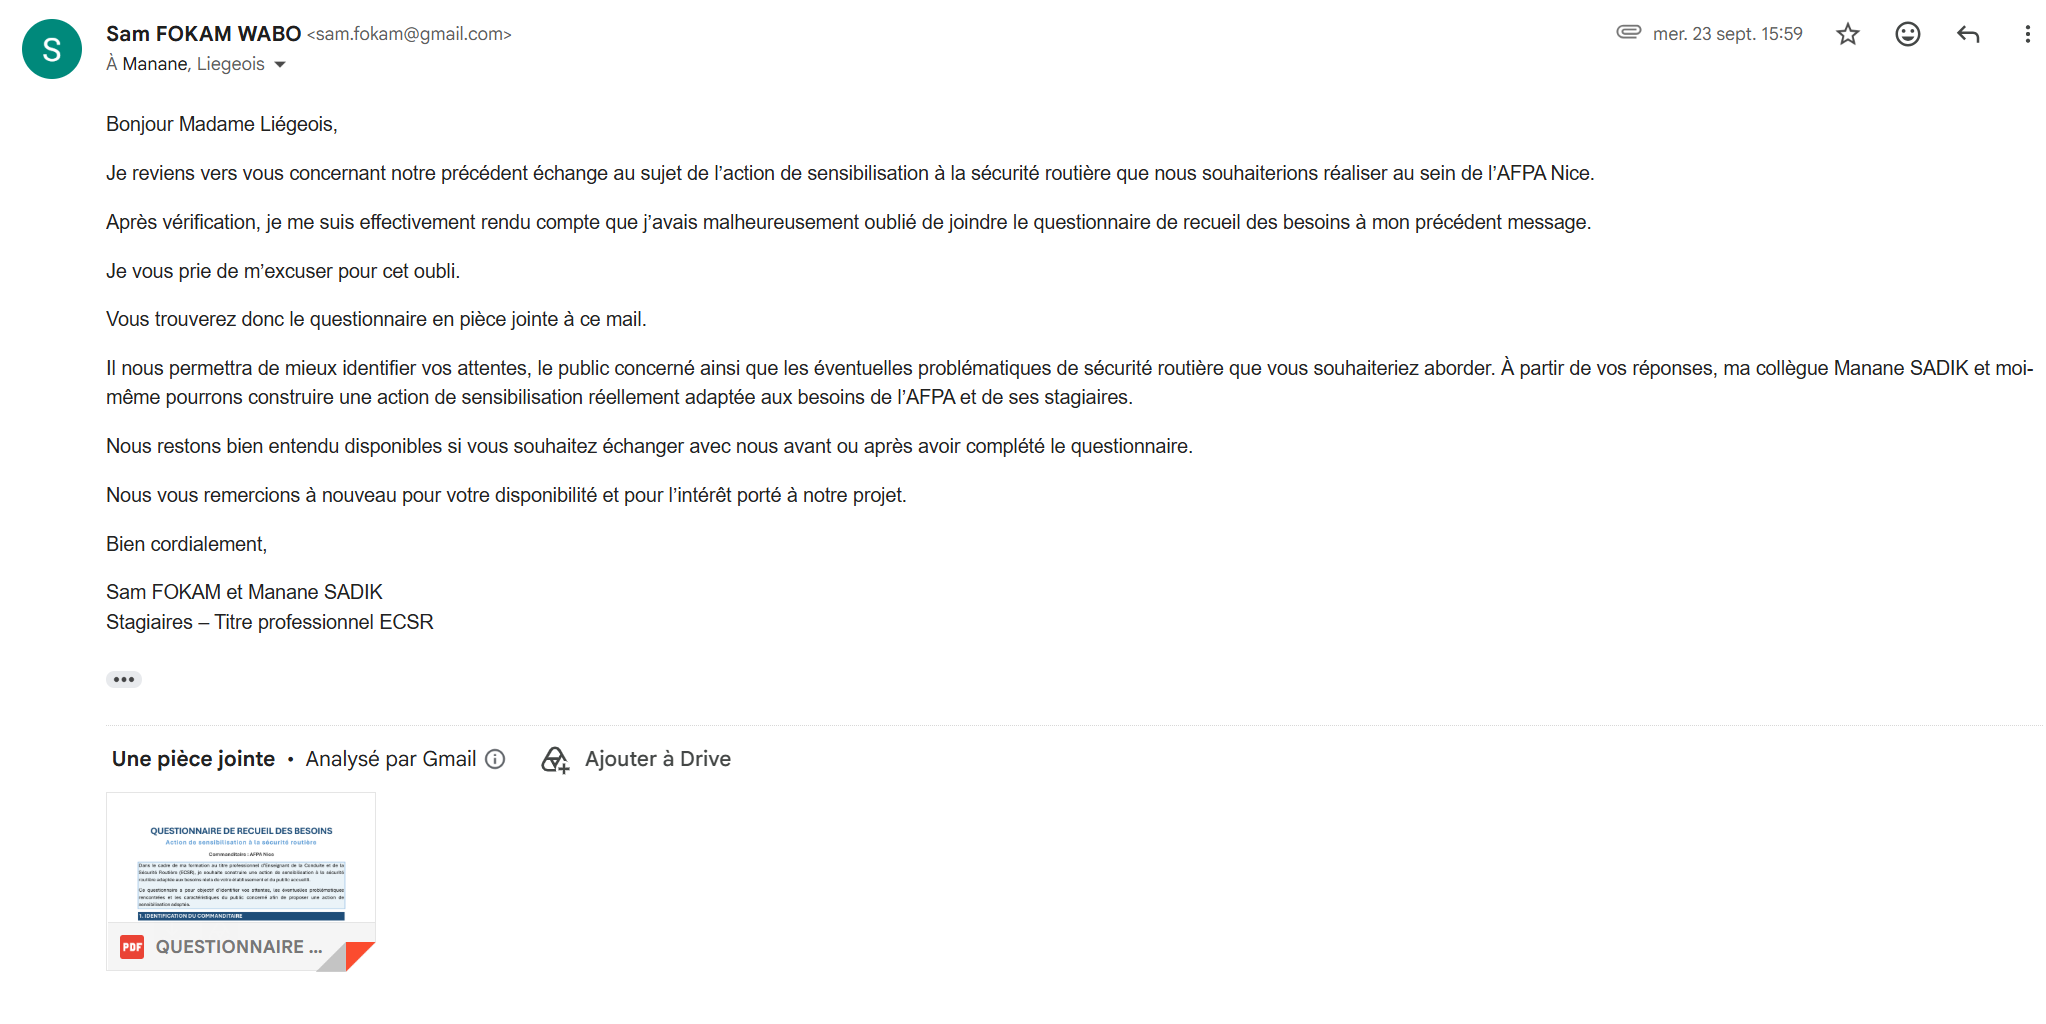
\includegraphics[width=0.97\linewidth,height=0.77\textheight,keepaspectratio]{images/annexes/echanges/a05_20260923_questionnaire.png}
\end{center}
\end{landscape}

\section{Questionnaire de recueil des besoins du commanditaire (A2)}
Les pages suivantes reproduisent, sous forme d'images, le questionnaire de recueil des besoins adressé au commanditaire AFPA. Cette pièce est directement liée à la partie consacrée à l'analyse de la demande et à la clarification du besoin.

\clearpage
\subsection*{Questionnaire commanditaire --- page 1}
\begin{figure}[H]
\centering
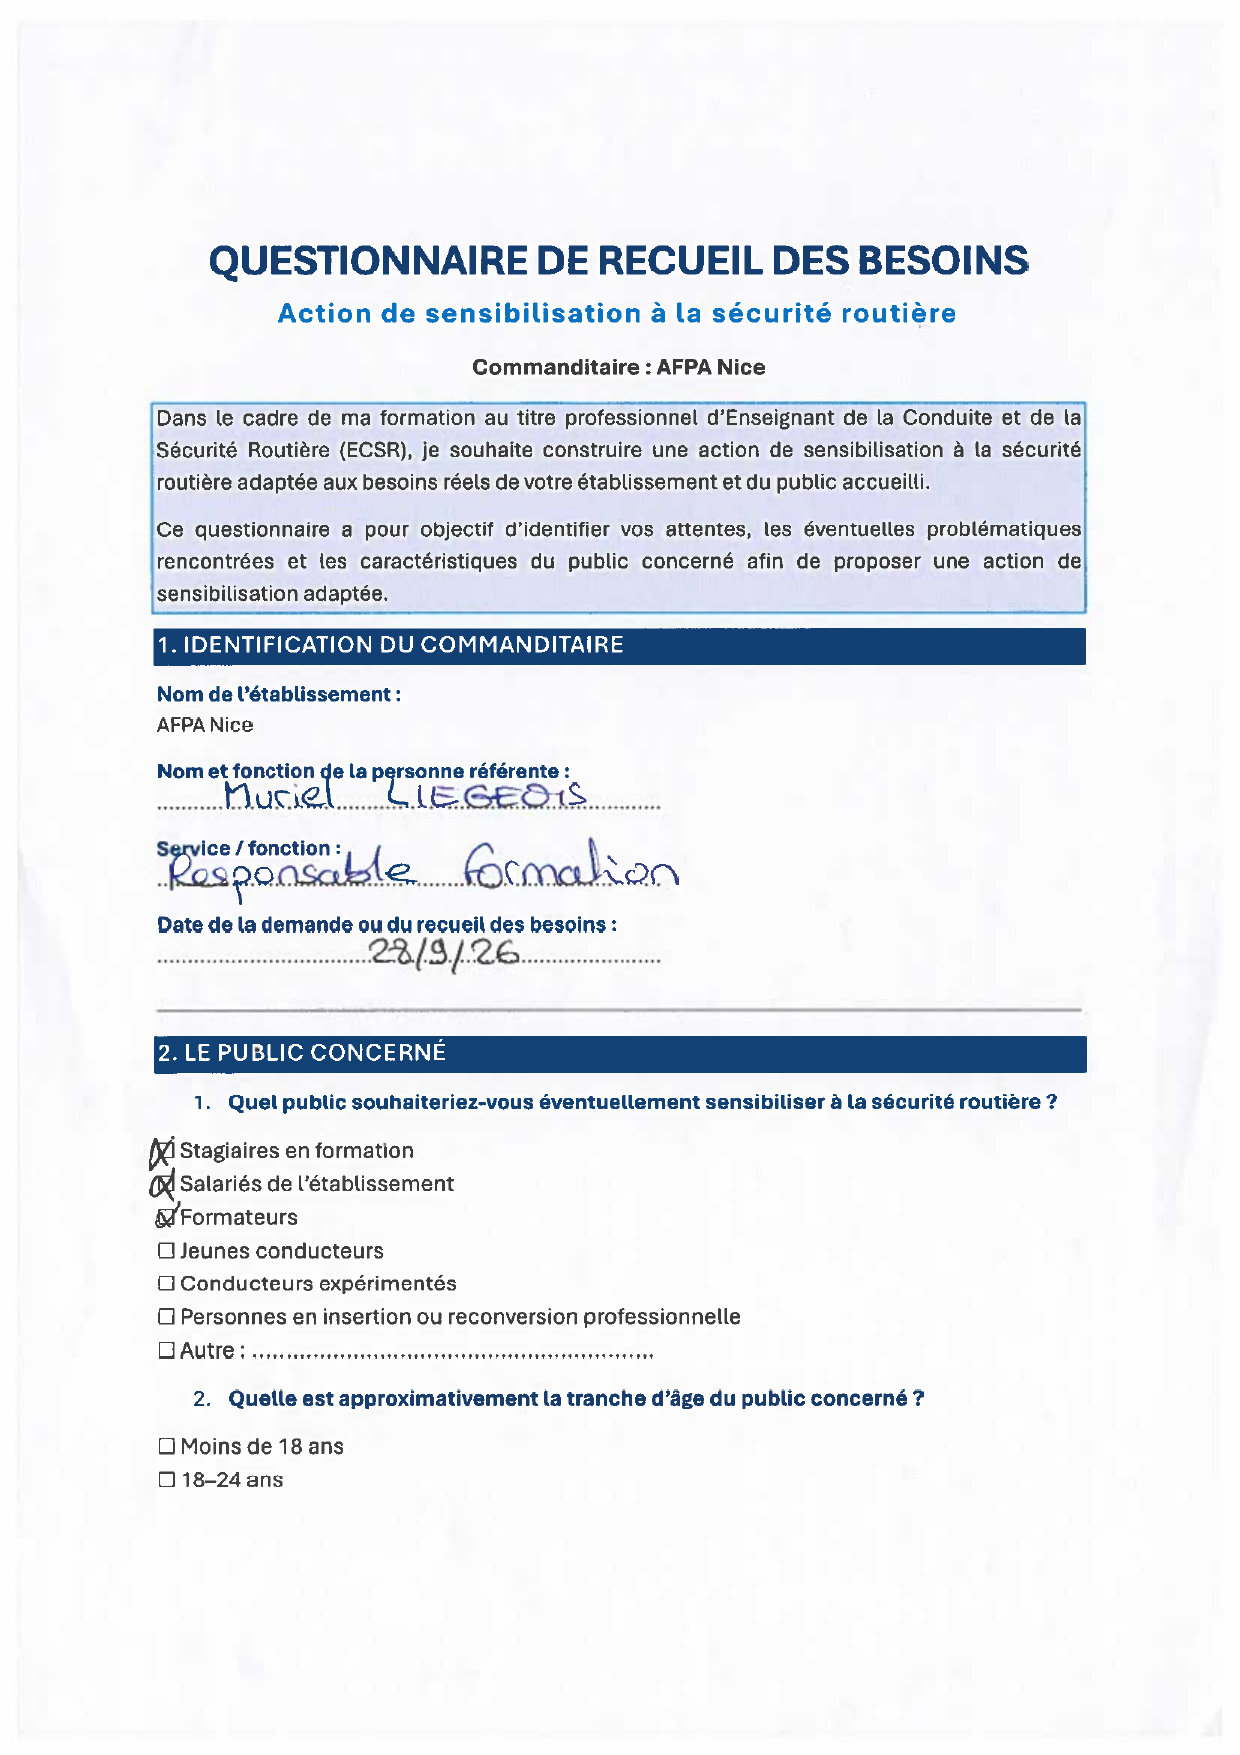
\includegraphics[width=0.92\textwidth]{images/annexes/questionnaire_commanditaire-1.png}
\end{figure}

\clearpage
\subsection*{Questionnaire commanditaire --- page 2}
\begin{figure}[H]
\centering
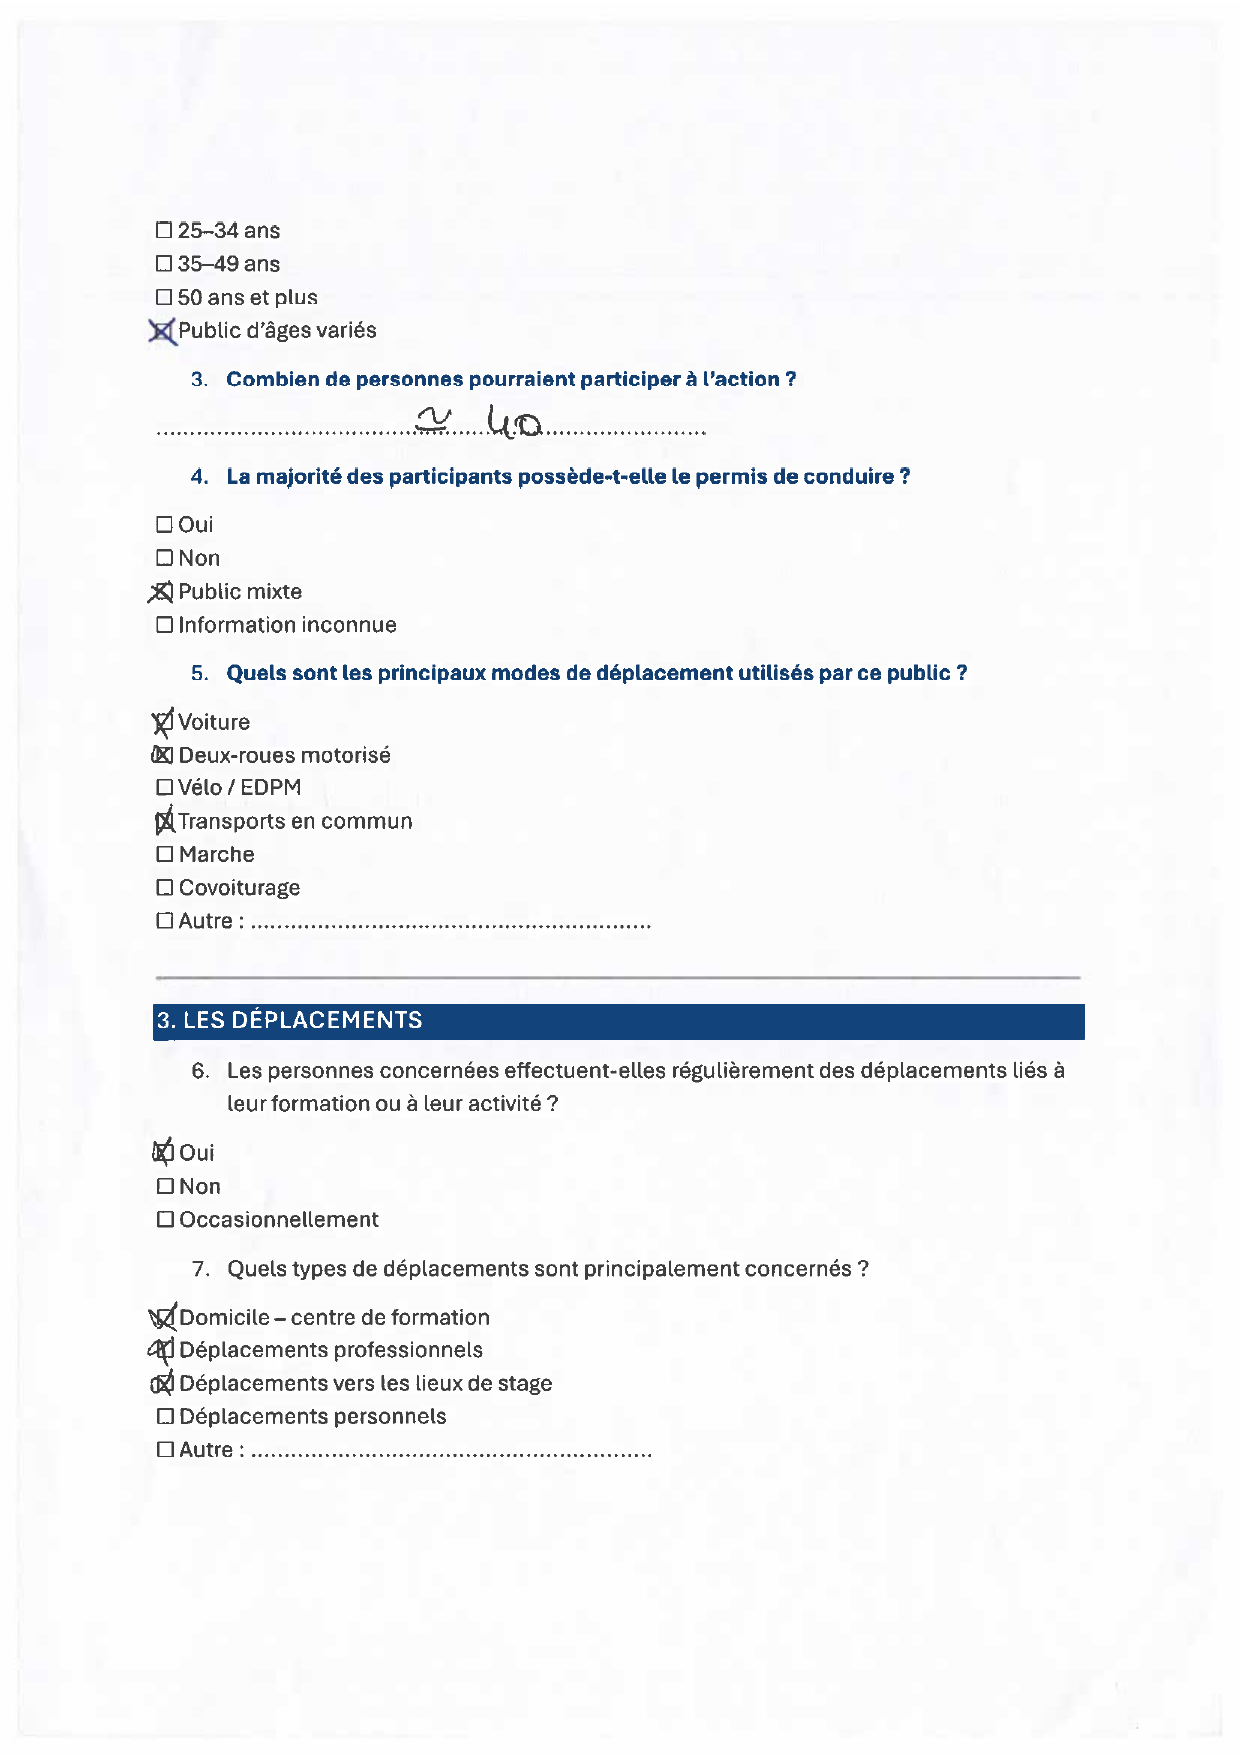
\includegraphics[width=0.92\textwidth]{images/annexes/questionnaire_commanditaire-2.png}
\end{figure}

\clearpage
\subsection*{Questionnaire commanditaire --- page 3}
\begin{figure}[H]
\centering
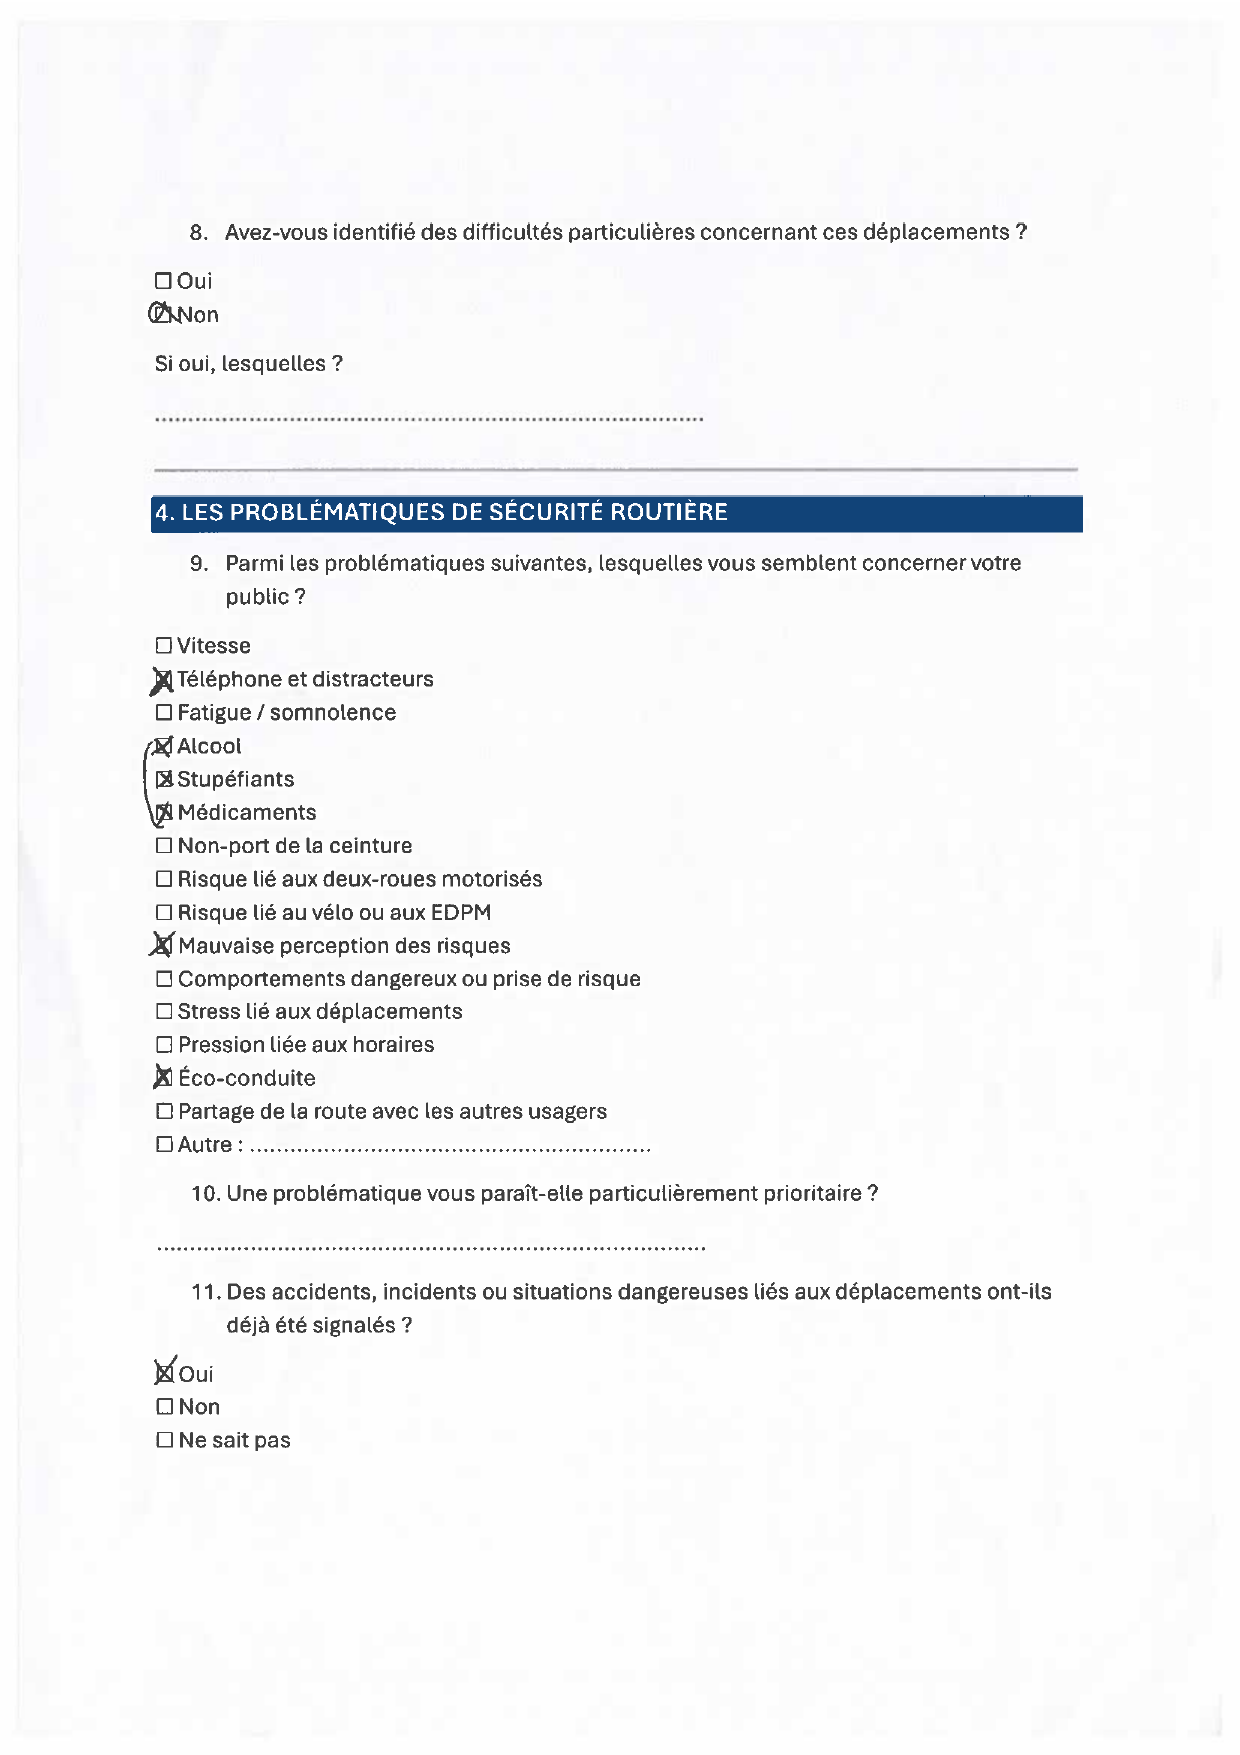
\includegraphics[width=0.92\textwidth]{images/annexes/questionnaire_commanditaire-3.png}
\end{figure}

\clearpage
\subsection*{Questionnaire commanditaire --- page 4}
\begin{figure}[H]
\centering
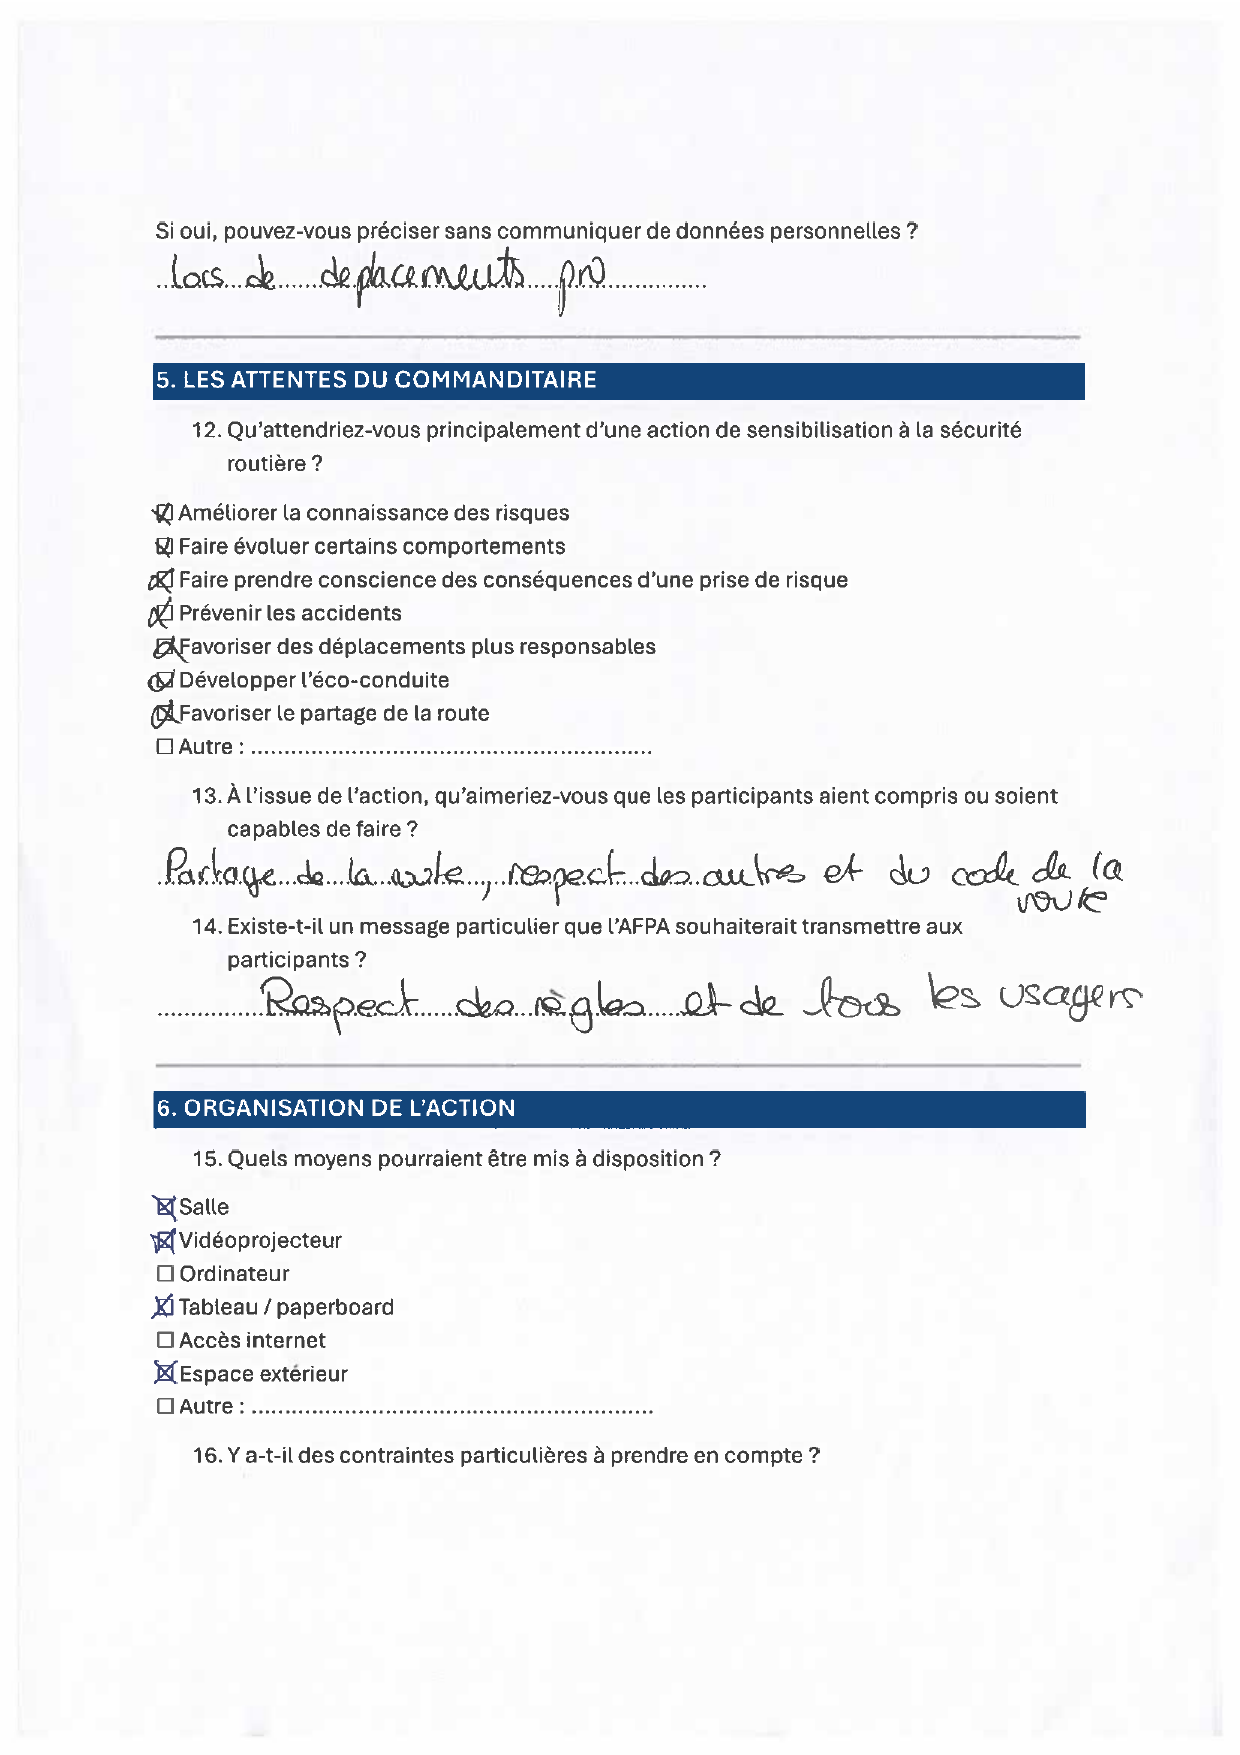
\includegraphics[width=0.92\textwidth]{images/annexes/questionnaire_commanditaire-4.png}
\end{figure}

\clearpage
\subsection*{Questionnaire commanditaire --- page 5}
\begin{figure}[H]
\centering
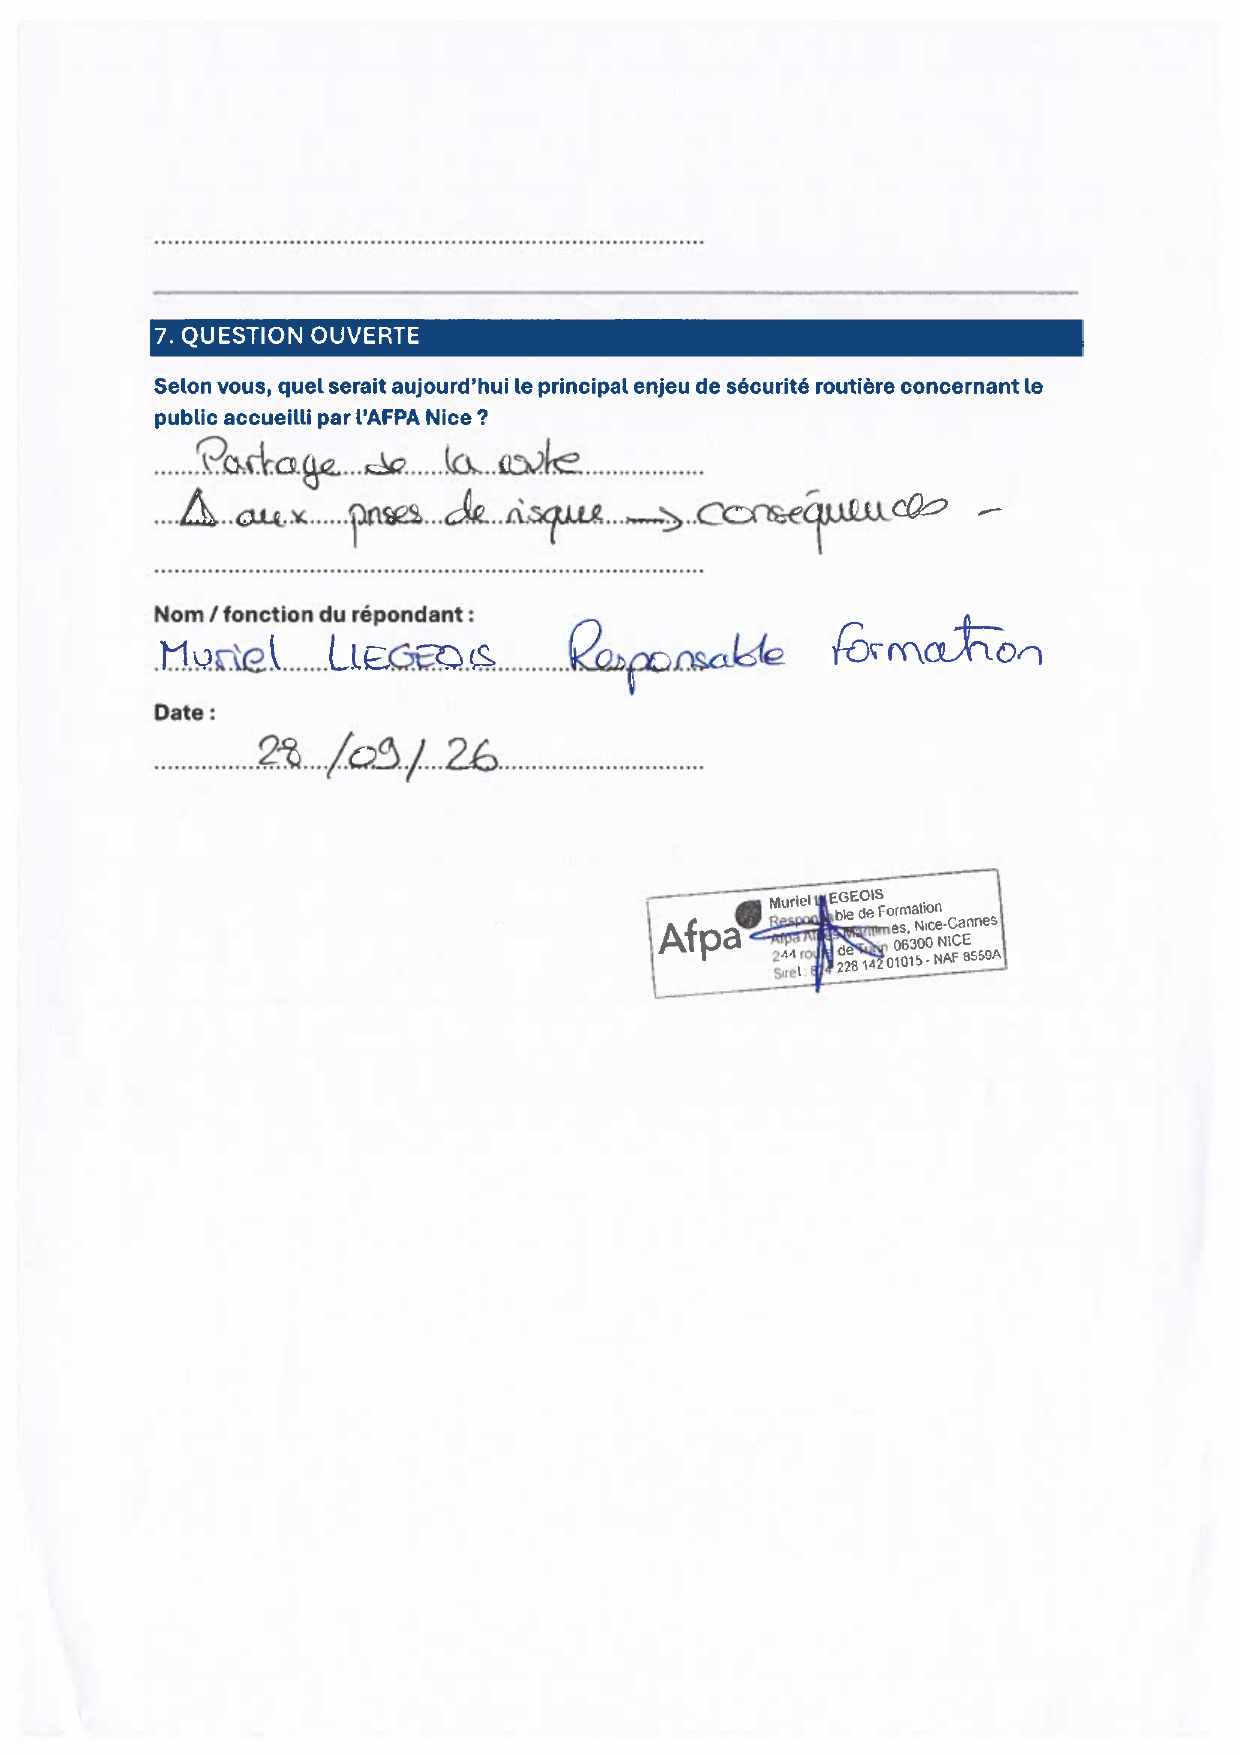
\includegraphics[width=0.92\textwidth]{images/annexes/questionnaire_commanditaire-5.png}
\end{figure}

\section{Échanges sur la clarification et le rendez-vous (A3)}
Ces pièces montrent les échanges autour de la réponse du commanditaire, de la date d’intervention et du rendez-vous du 1er octobre.

\clearpage
\begin{landscape}
\thispagestyle{plain}
\noindent{\large\bfseries 28 septembre — Retour annoncé et proposition d’intervention}\par\medskip
\begin{center}

\includegraphics[width=0.97\linewidth,height=0.77\textheight,keepaspectratio]{images/annexes/echanges/a06_20260928_reponse_afpa.png}
\end{center}
\end{landscape}

\clearpage
\begin{landscape}
\thispagestyle{plain}
\noindent{\large\bfseries 28 septembre — Demande d’entretien complémentaire}\par\medskip
\begin{center}
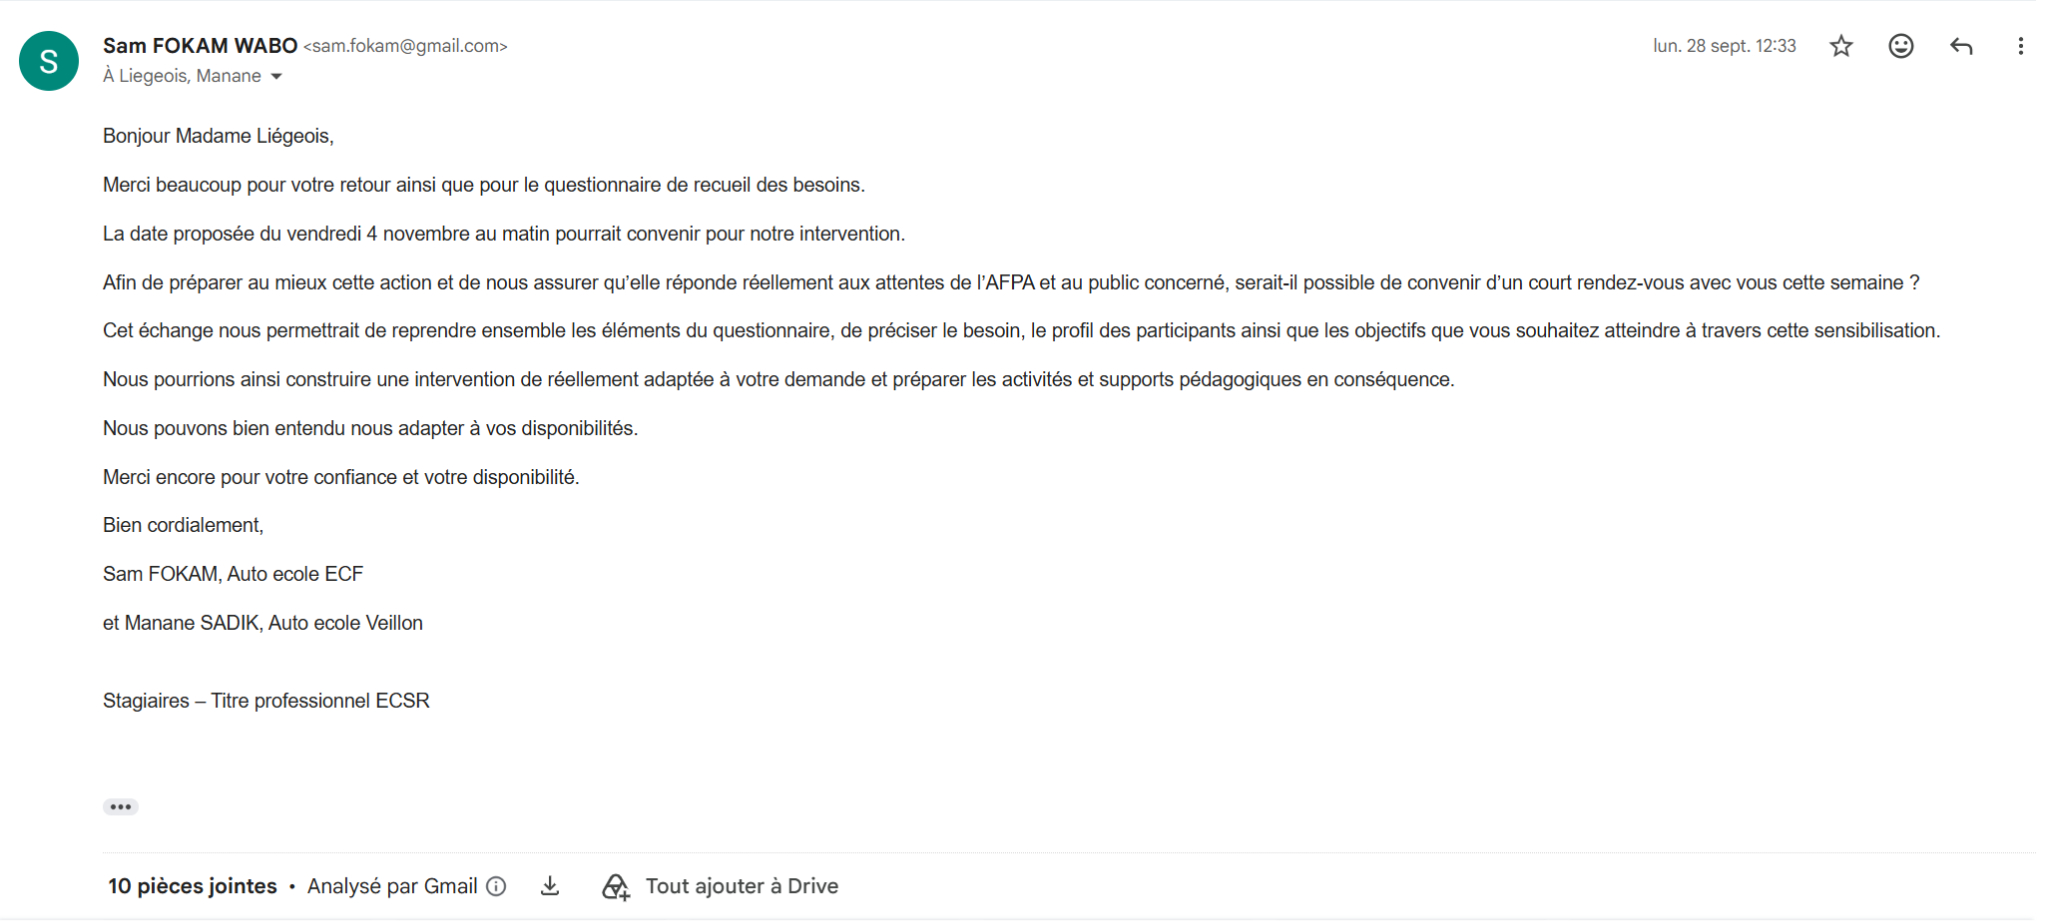
\includegraphics[width=0.97\linewidth,height=0.77\textheight,keepaspectratio]{images/annexes/echanges/a07_20260928_demande_rdv.png}
\end{center}
\end{landscape}

\clearpage
\begin{landscape}
\thispagestyle{plain}
\noindent{\large\bfseries 28 septembre — Rectification de la date et proposition de rendez-vous}\par\medskip
\begin{center}
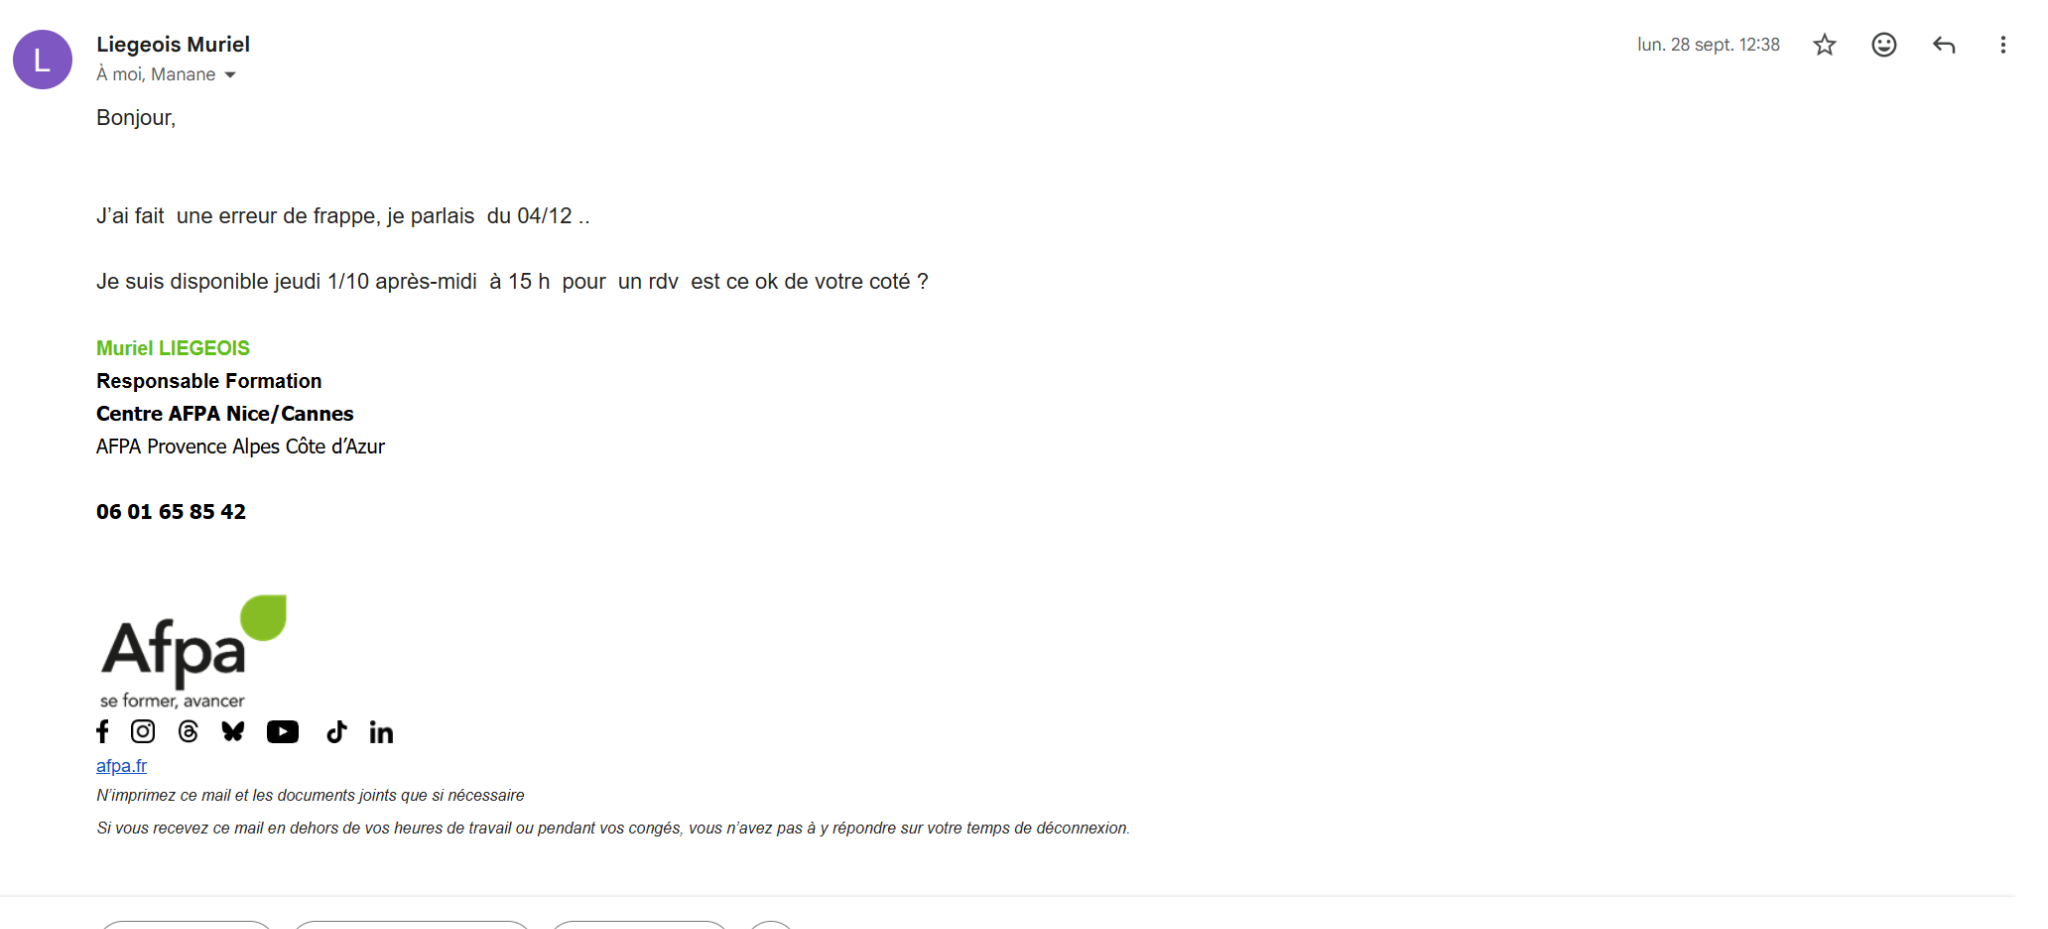
\includegraphics[width=0.97\linewidth,height=0.77\textheight,keepaspectratio]{images/annexes/echanges/a08_20260928_date_et_rdv.png}
\end{center}
\end{landscape}

\clearpage
\begin{landscape}
\thispagestyle{plain}
\noindent{\large\bfseries 28 septembre — Confirmation du rendez-vous}\par\medskip
\begin{center}

\includegraphics[width=0.97\linewidth,height=0.77\textheight,keepaspectratio]{images/annexes/echanges/a09_20260928_confirmation.png}
\end{center}
\end{landscape}

\clearpage
\begin{landscape}
\thispagestyle{plain}
\noindent{\large\bfseries 28 septembre — Invitation Outlook confirmée}\par\medskip
\begin{center}
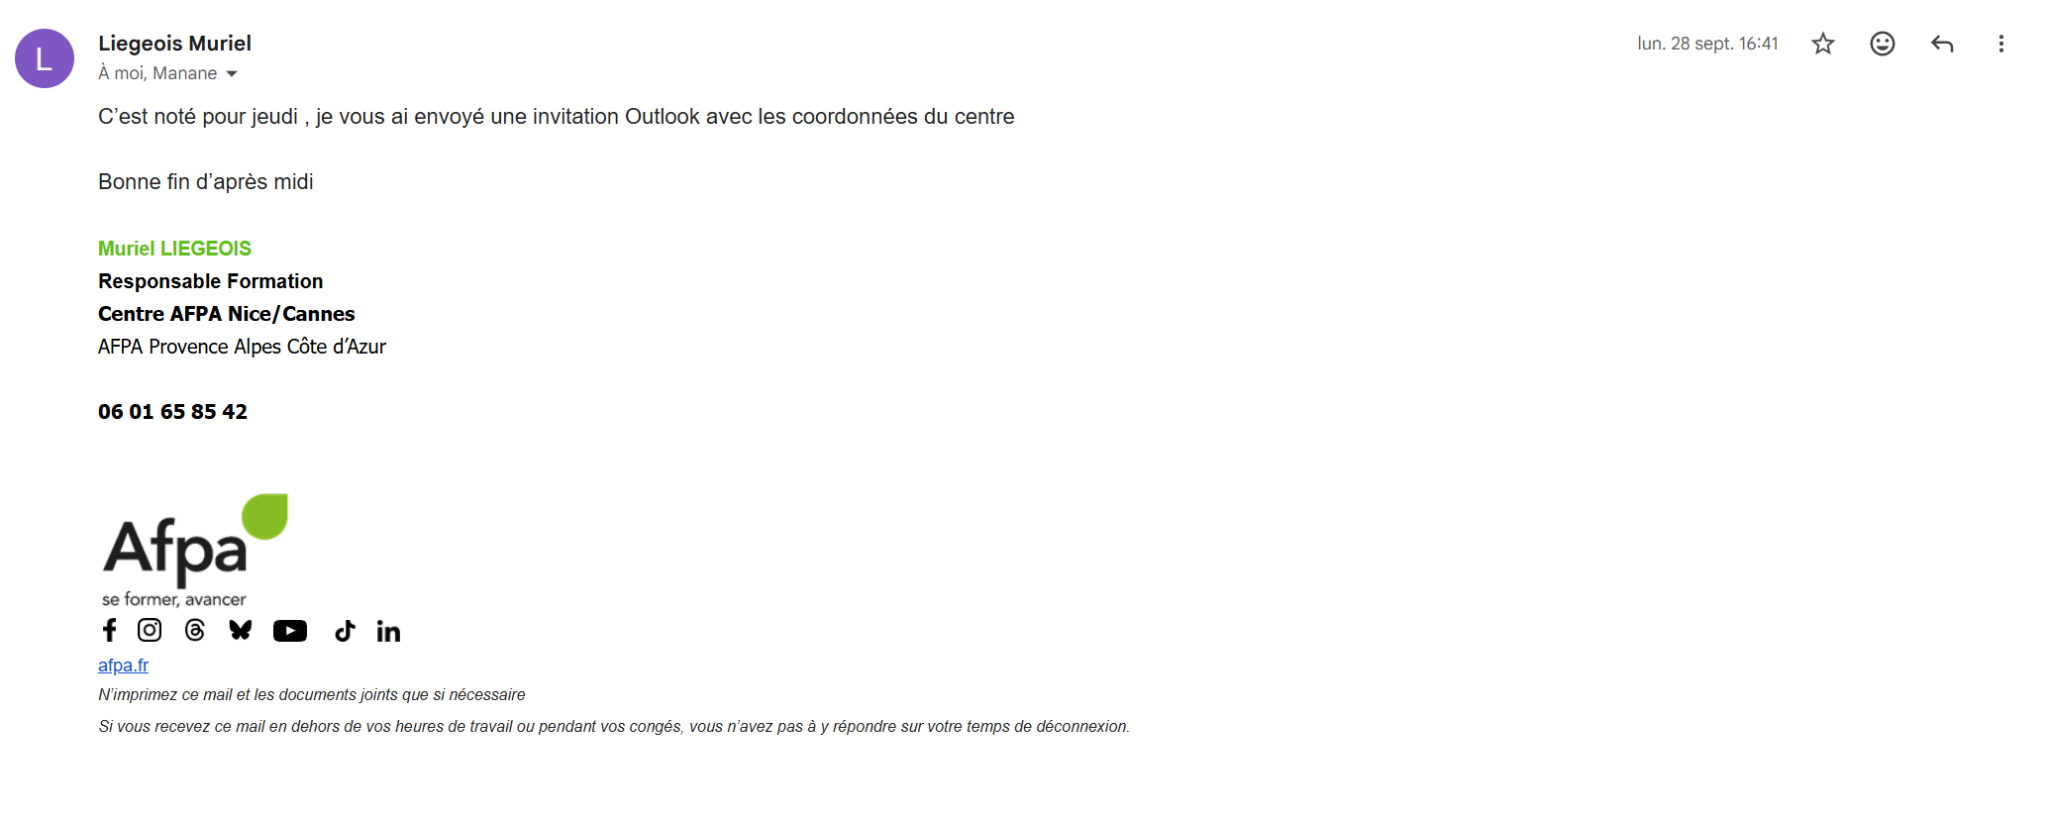
\includegraphics[width=0.97\linewidth,height=0.77\textheight,keepaspectratio]{images/annexes/echanges/a10_20260928_invitation.png}
\end{center}
\end{landscape}

\clearpage
\begin{landscape}
\thispagestyle{plain}
\noindent{\large\bfseries 28 septembre — Nouvelle demande de la pièce jointe}\par\medskip
\begin{center}

\includegraphics[width=0.97\linewidth,height=0.77\textheight,keepaspectratio]{images/annexes/echanges/a11_20260928_pj_absente.png}
\end{center}
\end{landscape}

\clearpage
\begin{landscape}
\thispagestyle{plain}
\noindent{\large\bfseries 29 septembre — Envoi effectif des réponses du commanditaire}\par\medskip
\begin{center}

\includegraphics[width=0.97\linewidth,height=0.77\textheight,keepaspectratio]{images/annexes/echanges/a12_20260929_questionnaire_recu.png}
\end{center}
\end{landscape}

\section{Questionnaire destiné aux stagiaires (A4)}
Les pages suivantes reproduisent, sous forme d'images, le questionnaire anonyme de trente questions destiné aux stagiaires plombiers de l'AFPA. Cette pièce correspond à la partie consacrée au diagnostic du public et à l'identification du besoin réel.

\clearpage
\subsection*{Questionnaire stagiaires --- page 1}
\begin{figure}[H]
\centering
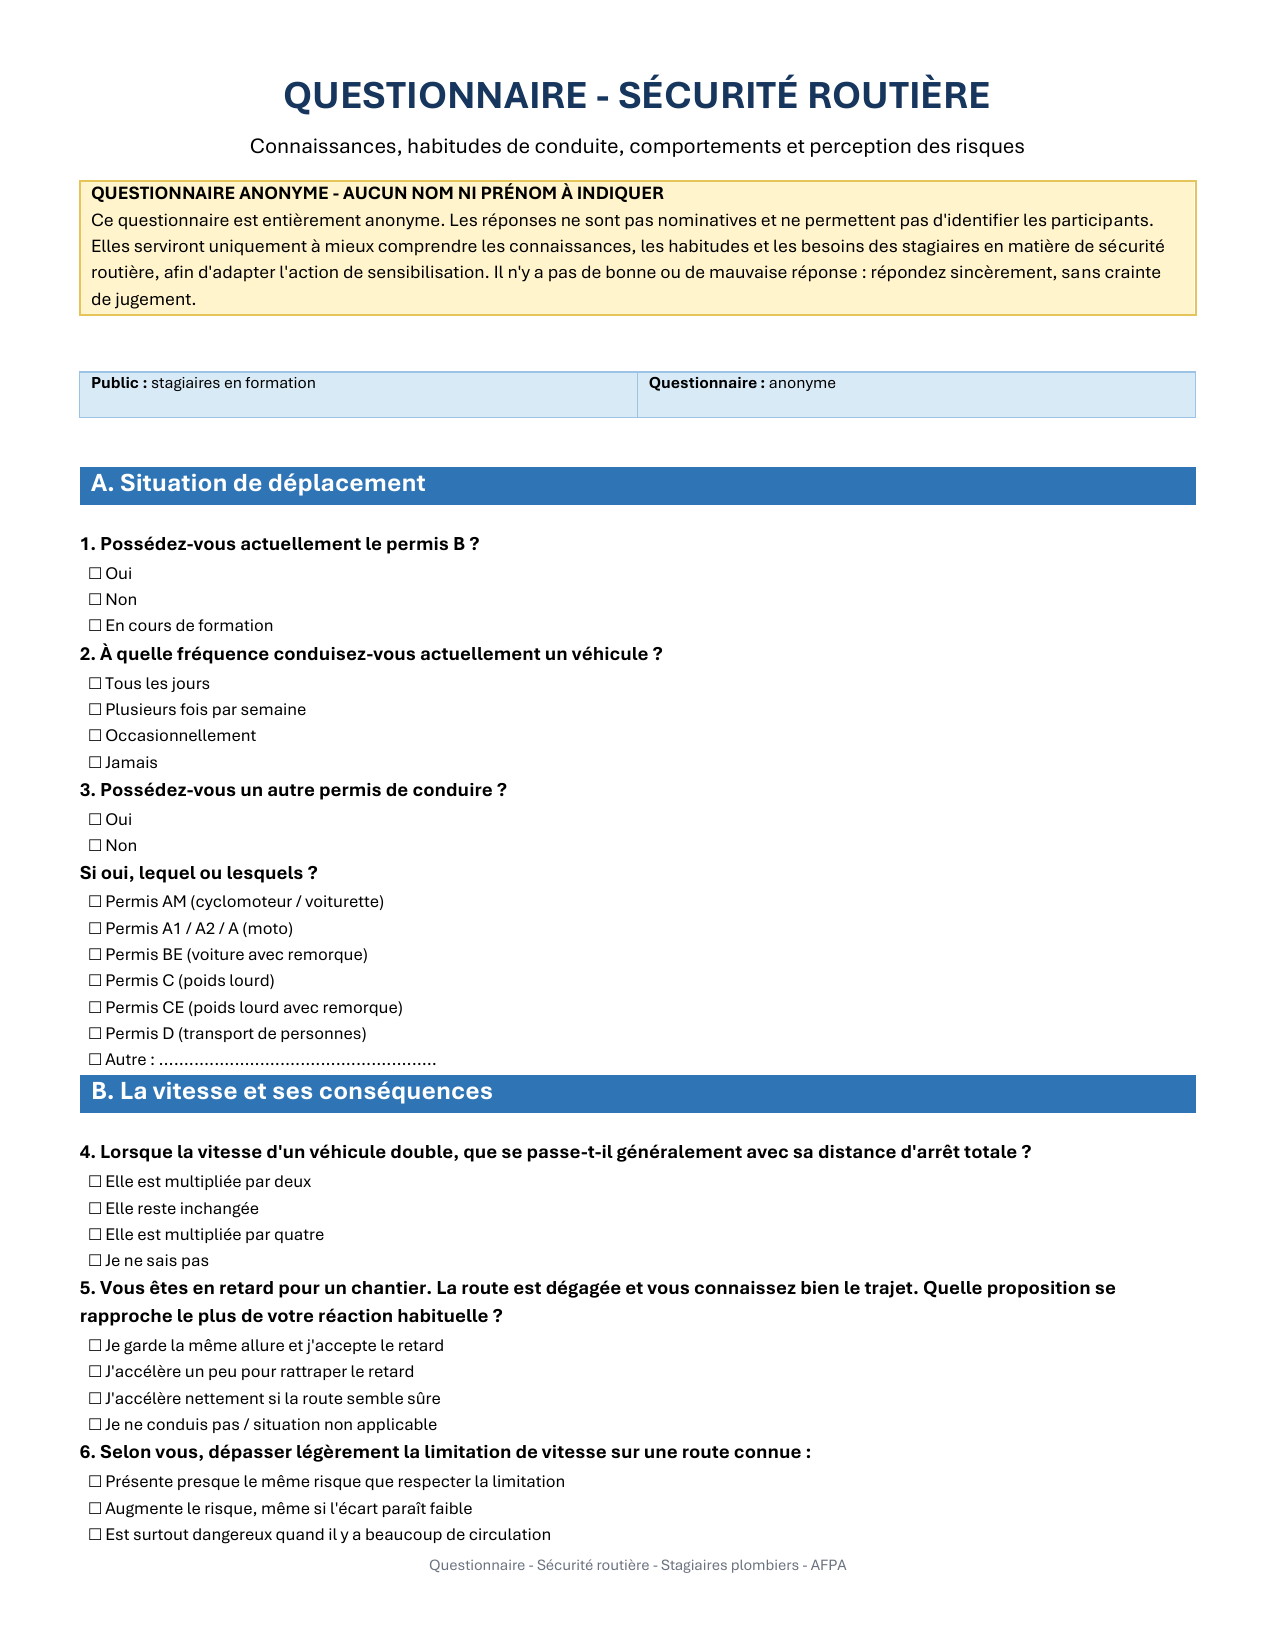
\includegraphics[width=0.92\textwidth]{images/annexes/questionnaire_stagiaires-1.png}
\end{figure}

\clearpage
\subsection*{Questionnaire stagiaires --- page 2}
\begin{figure}[H]
\centering
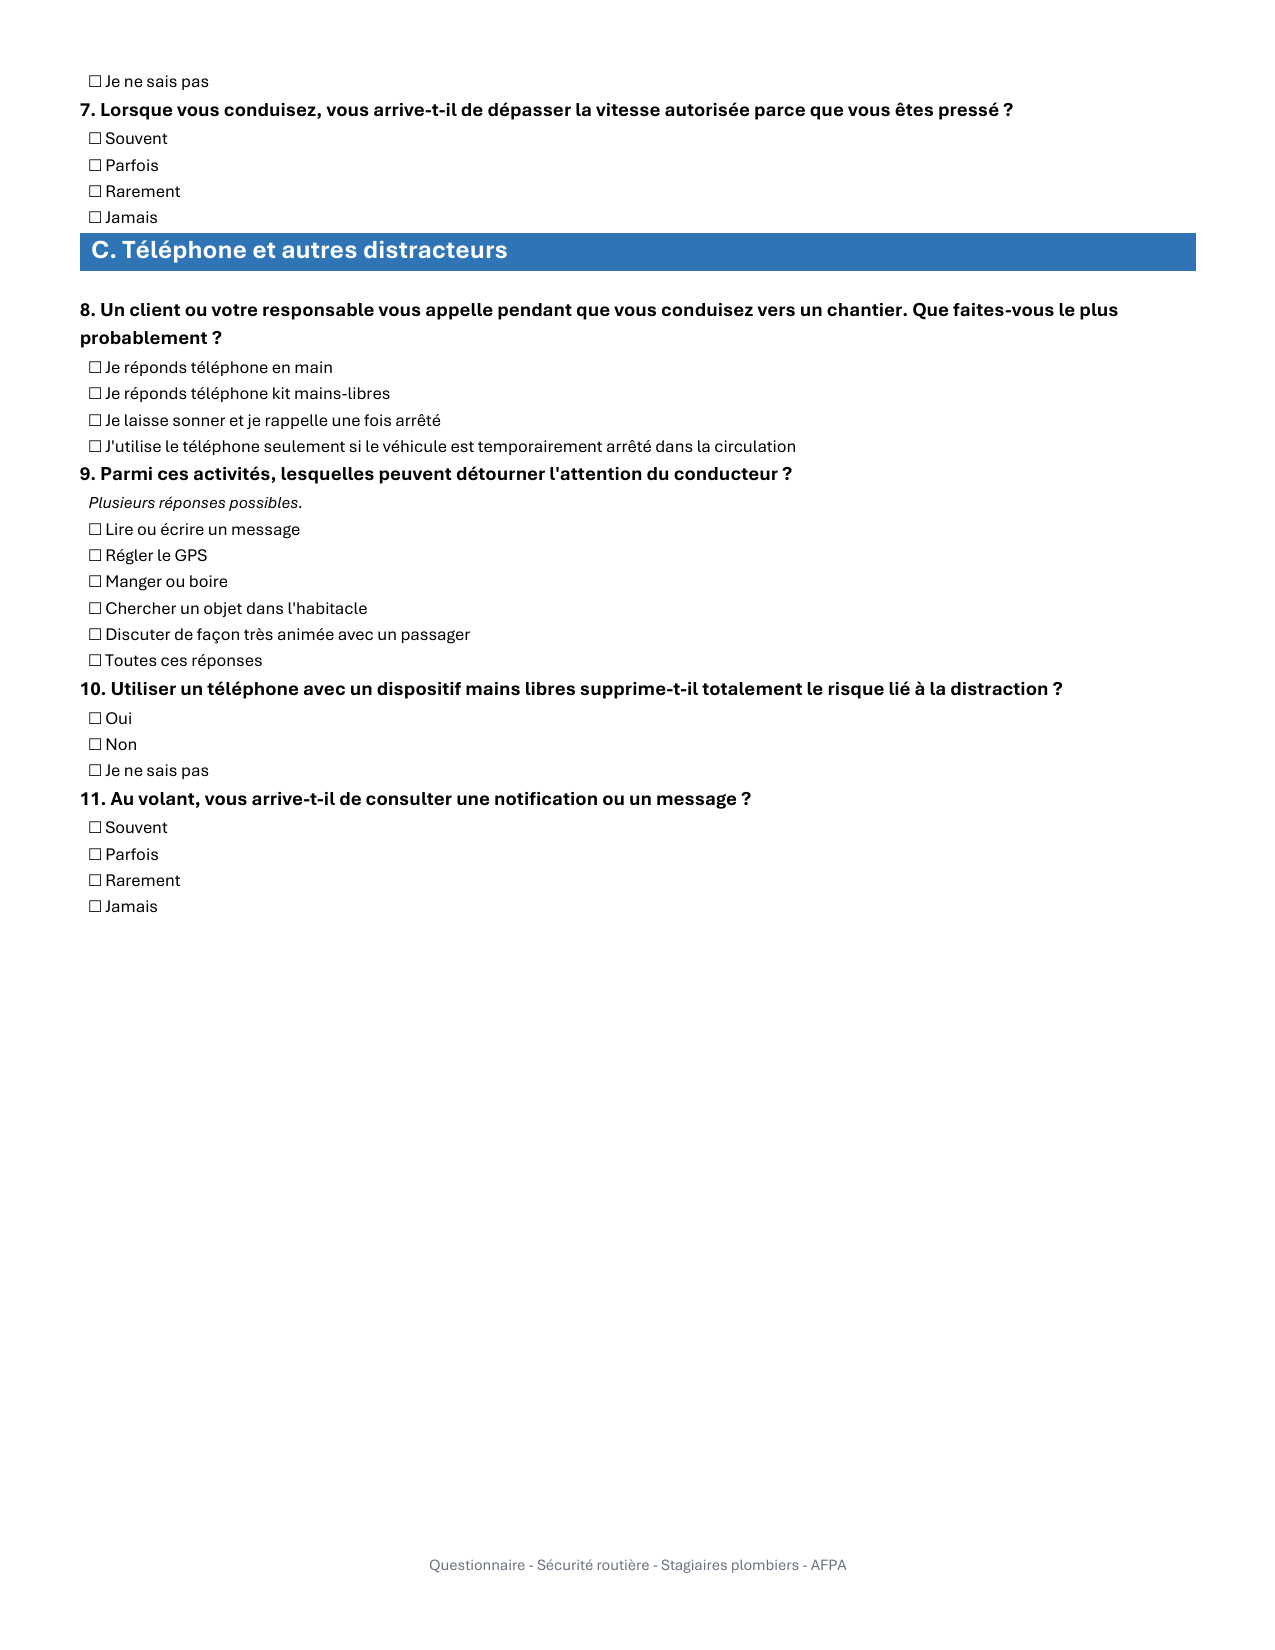
\includegraphics[width=0.92\textwidth]{images/annexes/questionnaire_stagiaires-2.png}
\end{figure}

\clearpage
\subsection*{Questionnaire stagiaires --- page 3}
\begin{figure}[H]
\centering
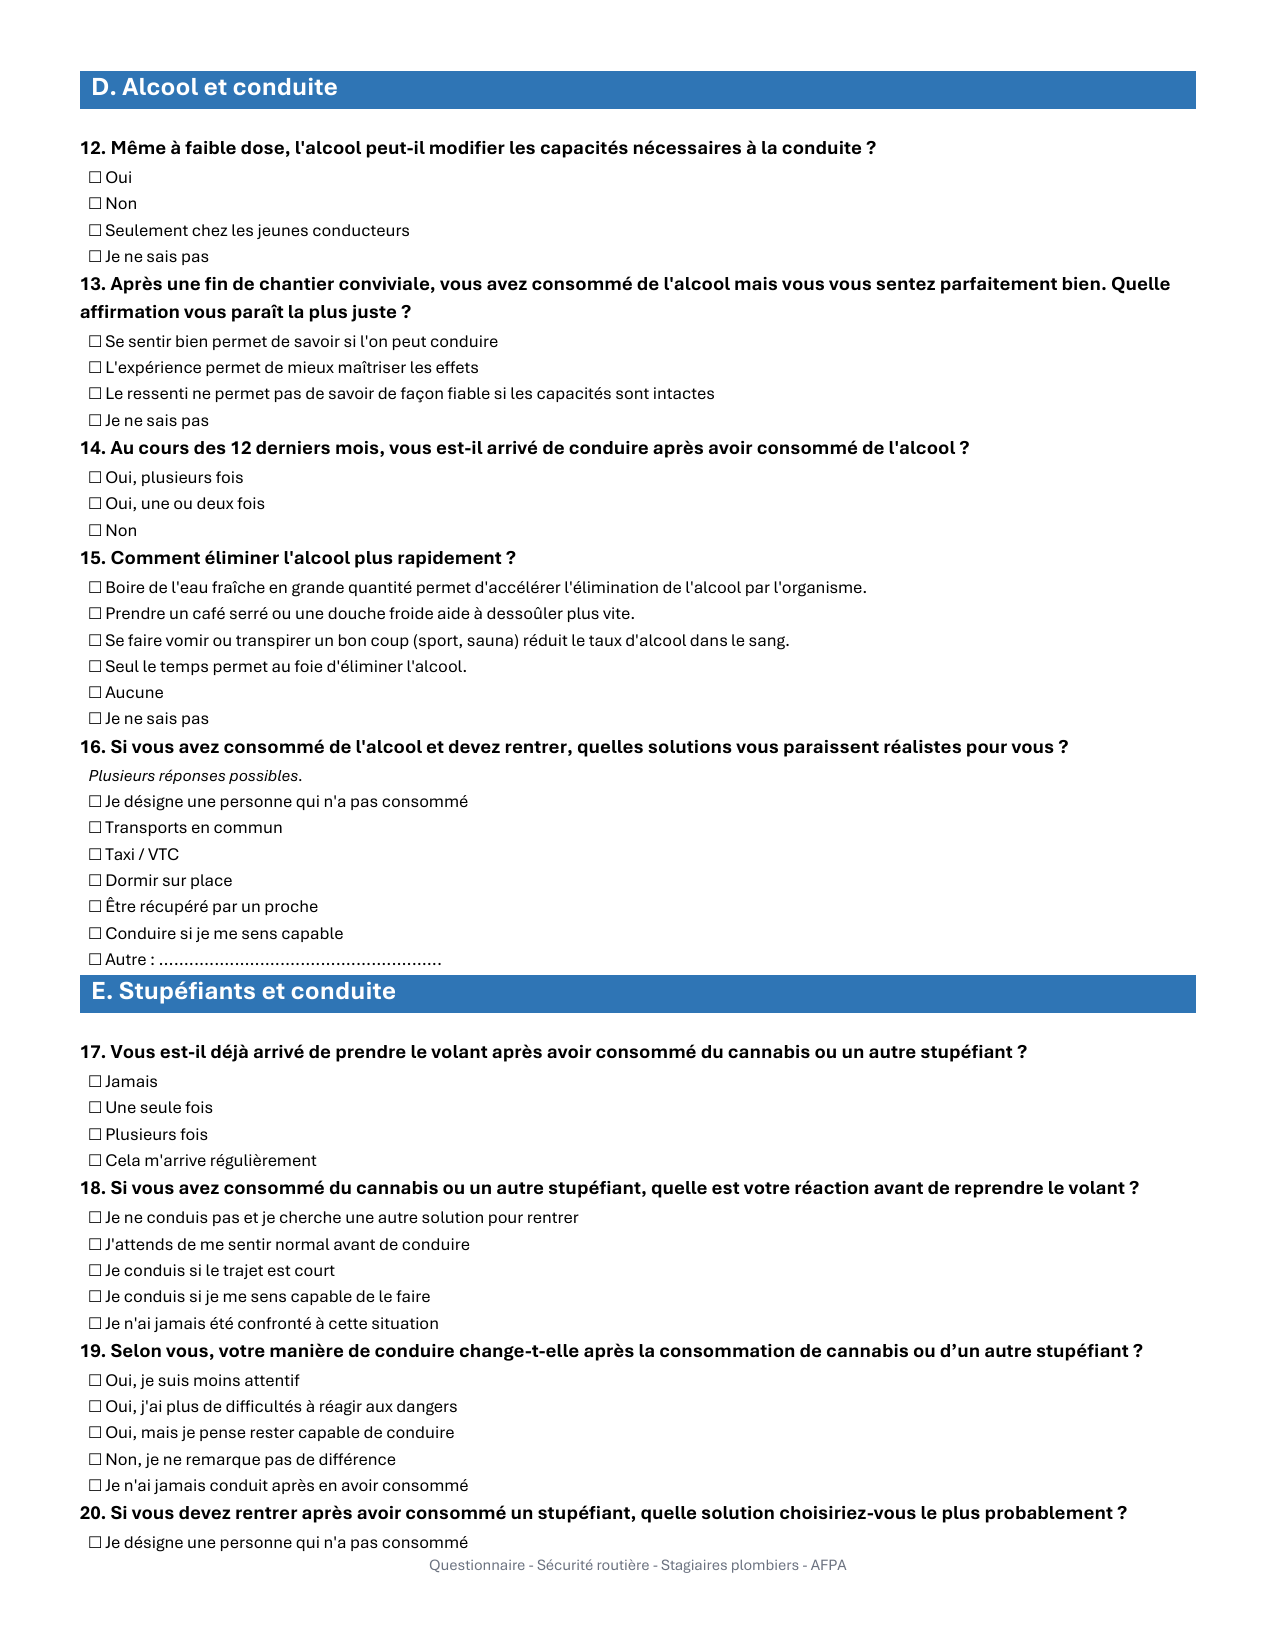
\includegraphics[width=0.92\textwidth]{images/annexes/questionnaire_stagiaires-3.png}
\end{figure}

\clearpage
\subsection*{Questionnaire stagiaires --- page 4}
\begin{figure}[H]
\centering
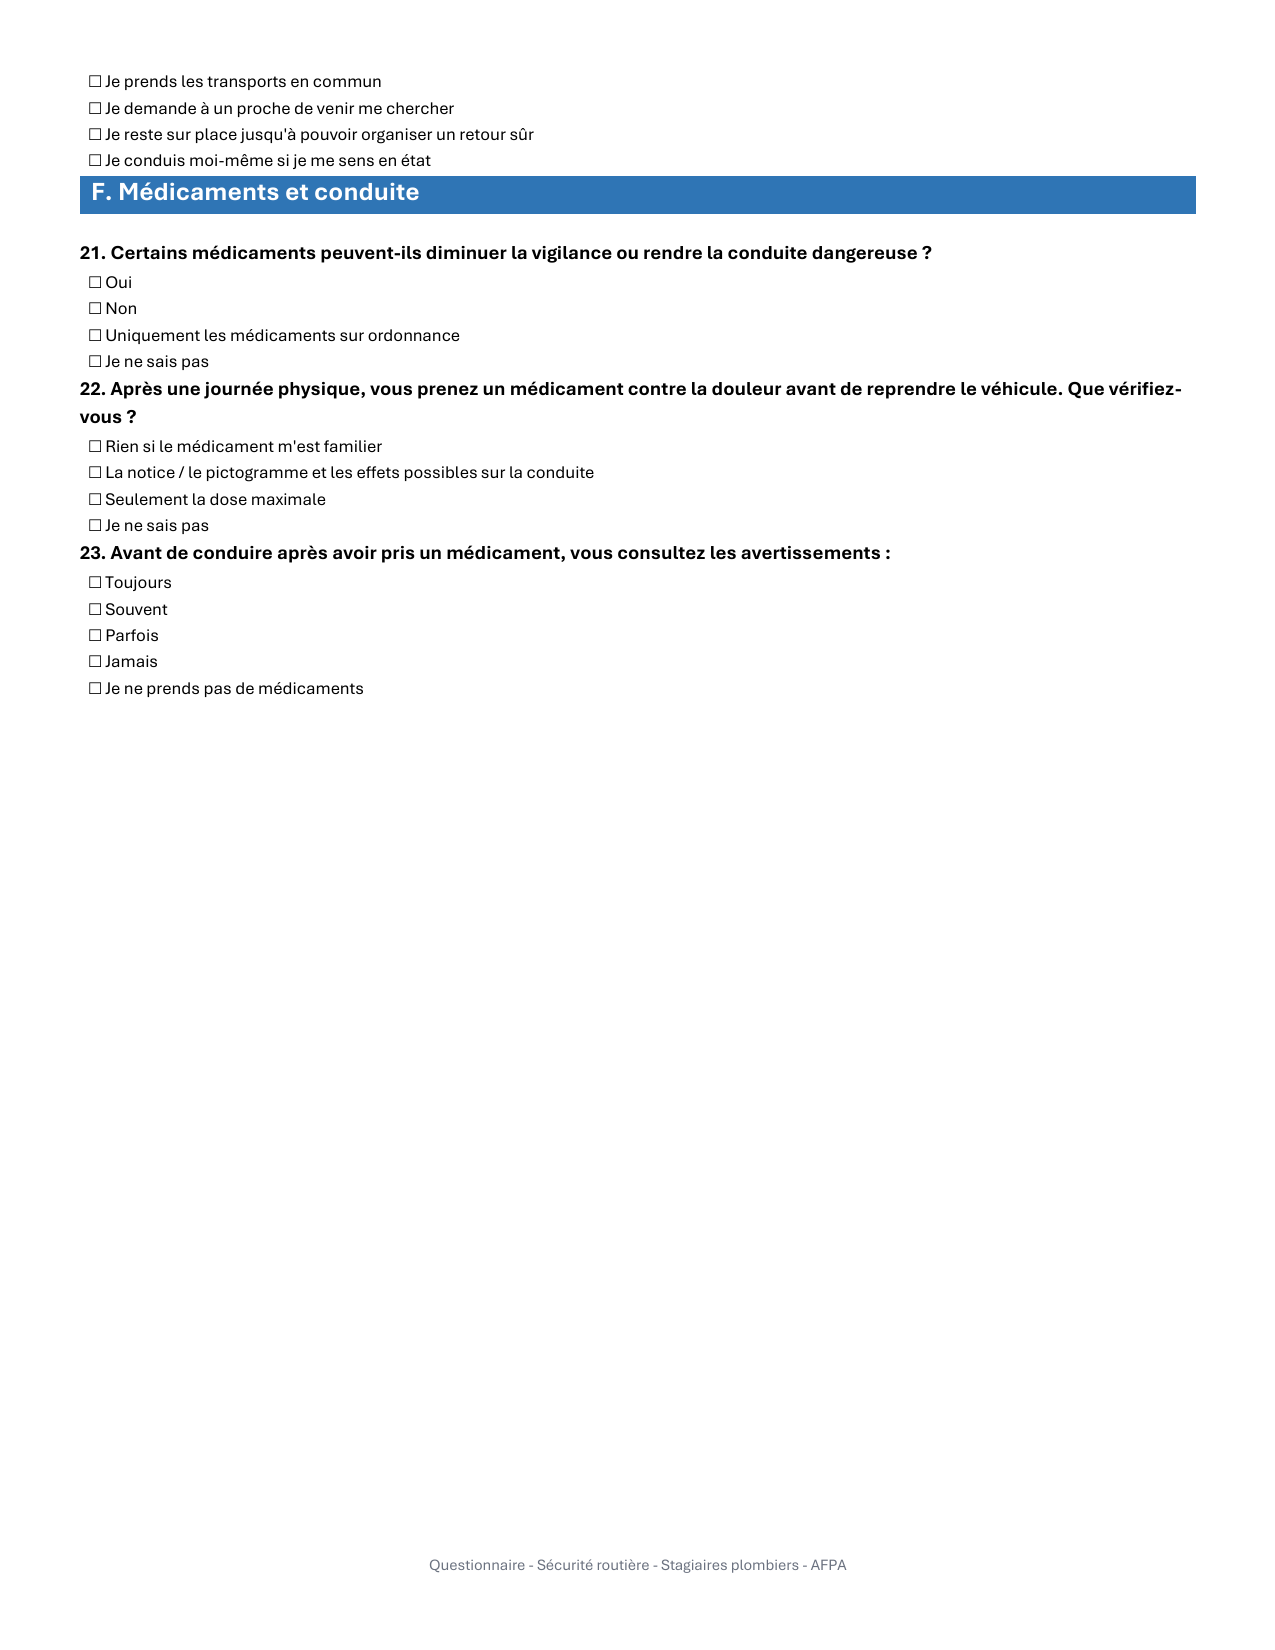
\includegraphics[width=0.92\textwidth]{images/annexes/questionnaire_stagiaires-4.png}
\end{figure}

\clearpage
\subsection*{Questionnaire stagiaires --- page 5}
\begin{figure}[H]
\centering
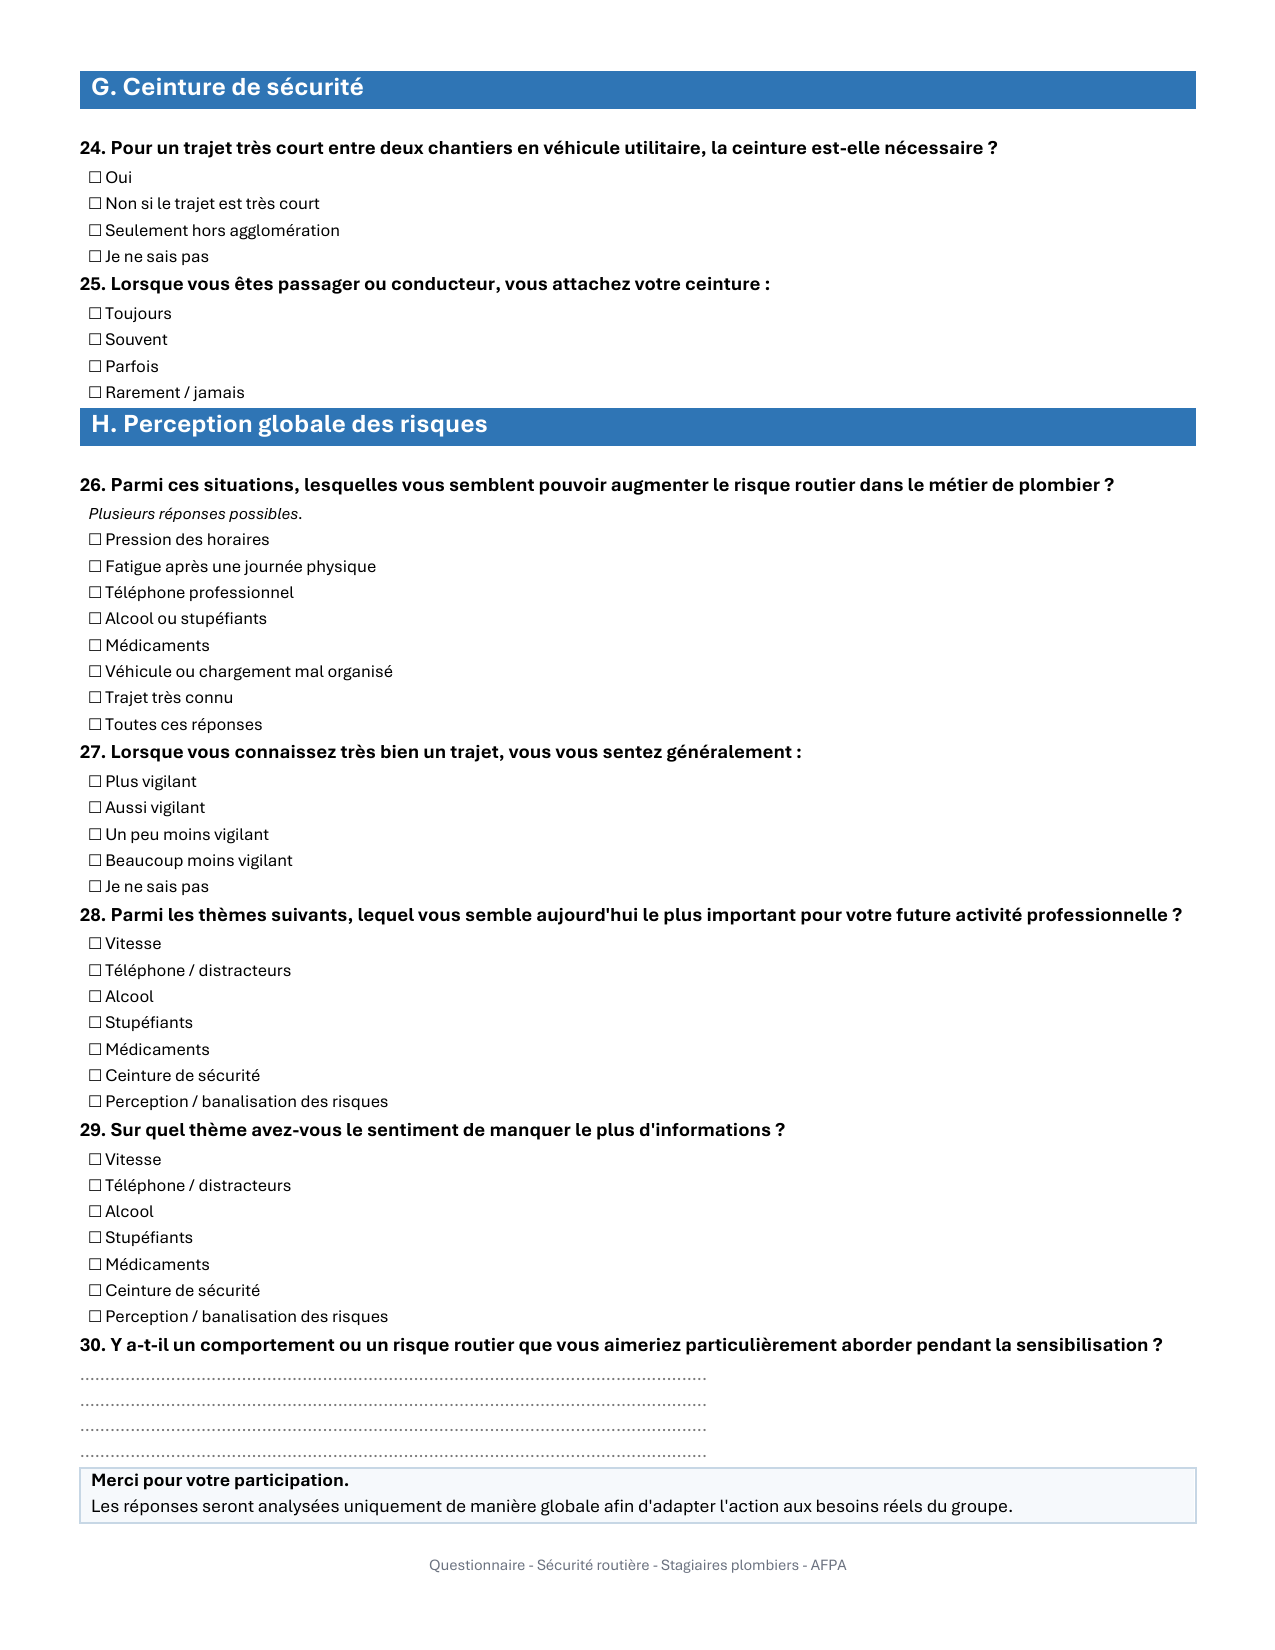
\includegraphics[width=0.92\textwidth]{images/annexes/questionnaire_stagiaires-5.png}
\end{figure}

\section{Échanges relatifs au questionnaire stagiaires (A5)}
Transmission, diffusion et relance du diagnostic auprès du groupe de stagiaires.

\clearpage
\begin{landscape}
\thispagestyle{plain}
\noindent{\large\bfseries 26 octobre — Transmission du questionnaire aux stagiaires}\par\medskip
\begin{center}

\includegraphics[width=0.97\linewidth,height=0.77\textheight,keepaspectratio]{images/annexes/echanges/a13_20261026_questionnaire_stagiaires.png}
\end{center}
\end{landscape}

\clearpage
\begin{landscape}
\thispagestyle{plain}
\noindent{\large\bfseries 26 octobre — Accord de diffusion au groupe}\par\medskip
\begin{center}

\includegraphics[width=0.97\linewidth,height=0.77\textheight,keepaspectratio]{images/annexes/echanges/a14_20261026_accord_diffusion.png}
\end{center}
\end{landscape}

\clearpage
\begin{landscape}
\thispagestyle{plain}
\noindent{\large\bfseries 29 octobre — Relance pour les réponses}\par\medskip
\begin{center}

\includegraphics[width=0.97\linewidth,height=0.77\textheight,keepaspectratio]{images/annexes/echanges/a15_20261029_relance.png}
\end{center}
\end{landscape}

\clearpage
\begin{landscape}
\thispagestyle{plain}
\noindent{\large\bfseries 29 octobre — Réponse du commanditaire sur la numérisation}\par\medskip
\begin{center}

\includegraphics[width=0.97\linewidth,height=0.77\textheight,keepaspectratio]{images/annexes/echanges/a16_20261029_confirmation_retour.png}
\end{center}
\end{landscape}

\section{Recherche de matériel auprès de la Préfecture (A7)}
Correspondance avec le Bureau de la sécurité routière et démarche initiale de conventionnement.

\clearpage
\begin{landscape}
\thispagestyle{plain}
\noindent{\large\bfseries 11 octobre — Sollicitation du Bureau de la sécurité routière}\par\medskip
\begin{center}
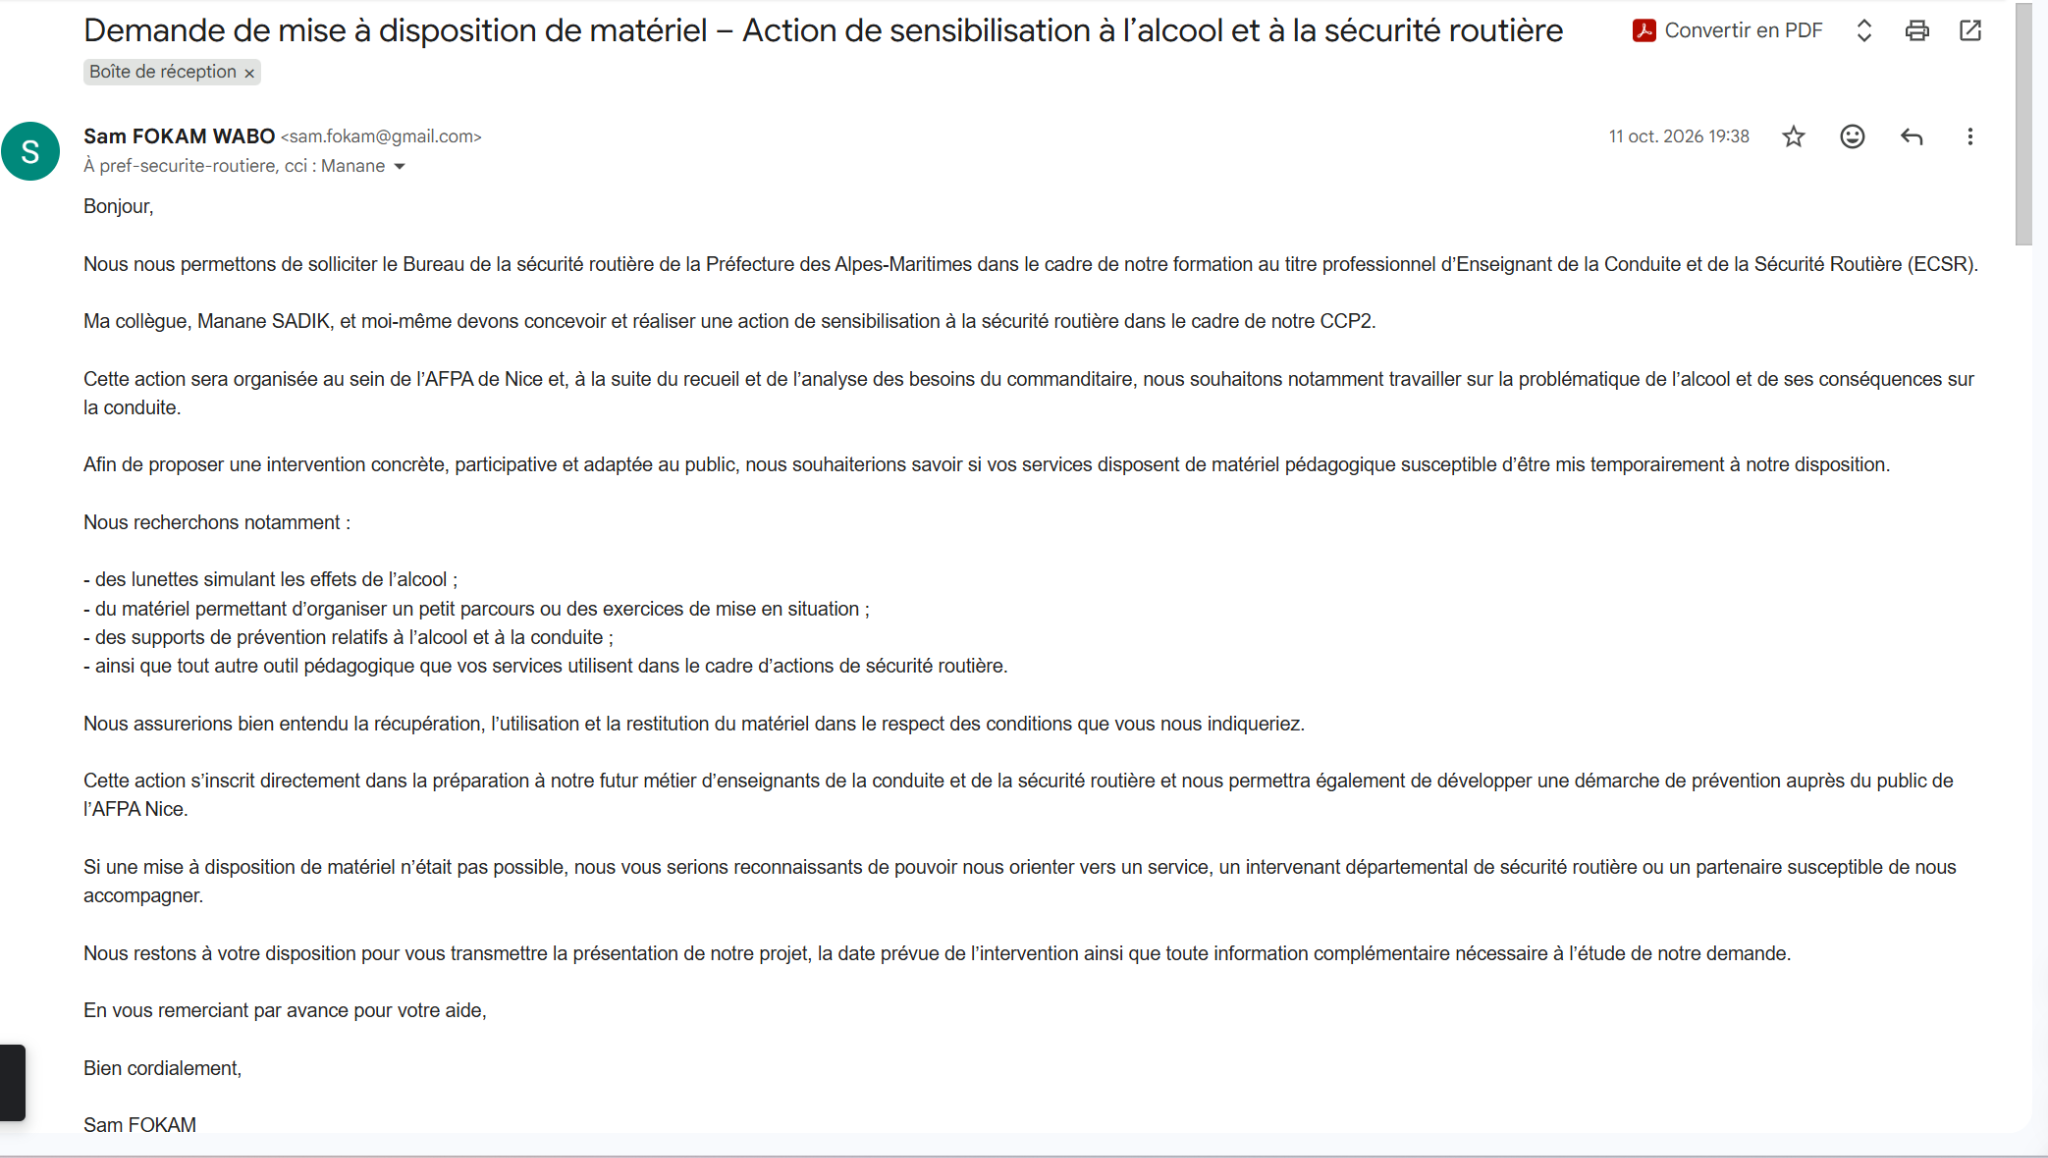
\includegraphics[width=0.97\linewidth,height=0.77\textheight,keepaspectratio]{images/annexes/echanges/p01_20261011_demande_materiel.png}
\end{center}
\end{landscape}

\clearpage
\begin{landscape}
\thispagestyle{plain}
\noindent{\large\bfseries 12 octobre — Proposition de matériel par la Préfecture}\par\medskip
\begin{center}
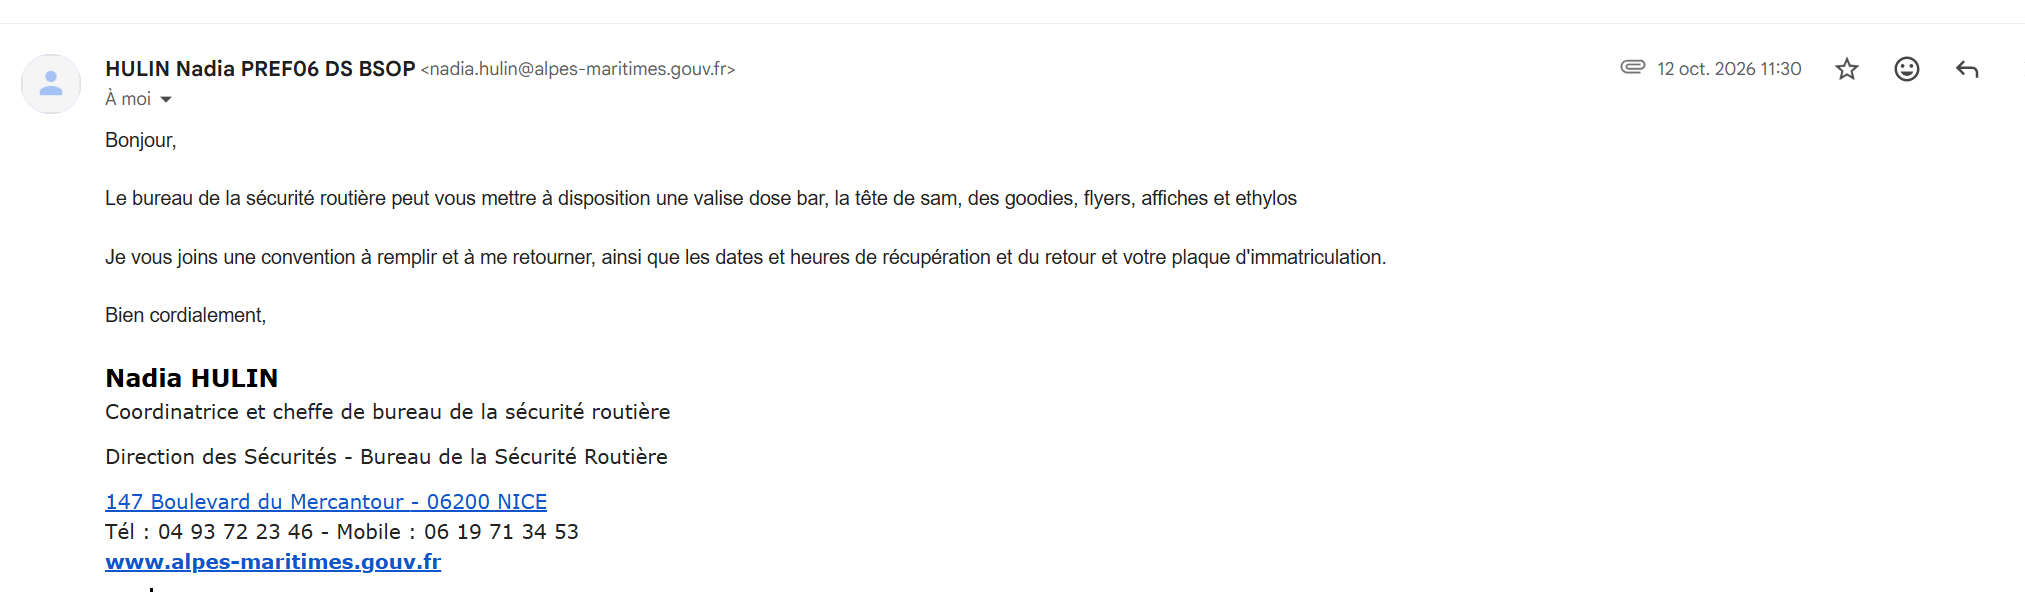
\includegraphics[width=0.97\linewidth,height=0.77\textheight,keepaspectratio]{images/annexes/echanges/p02_20261012_reponse_prefecture.png}
\end{center}
\end{landscape}

\clearpage
\begin{landscape}
\thispagestyle{plain}
\noindent{\large\bfseries 30 octobre — Envoi de la convention signée}\par\medskip
\begin{center}
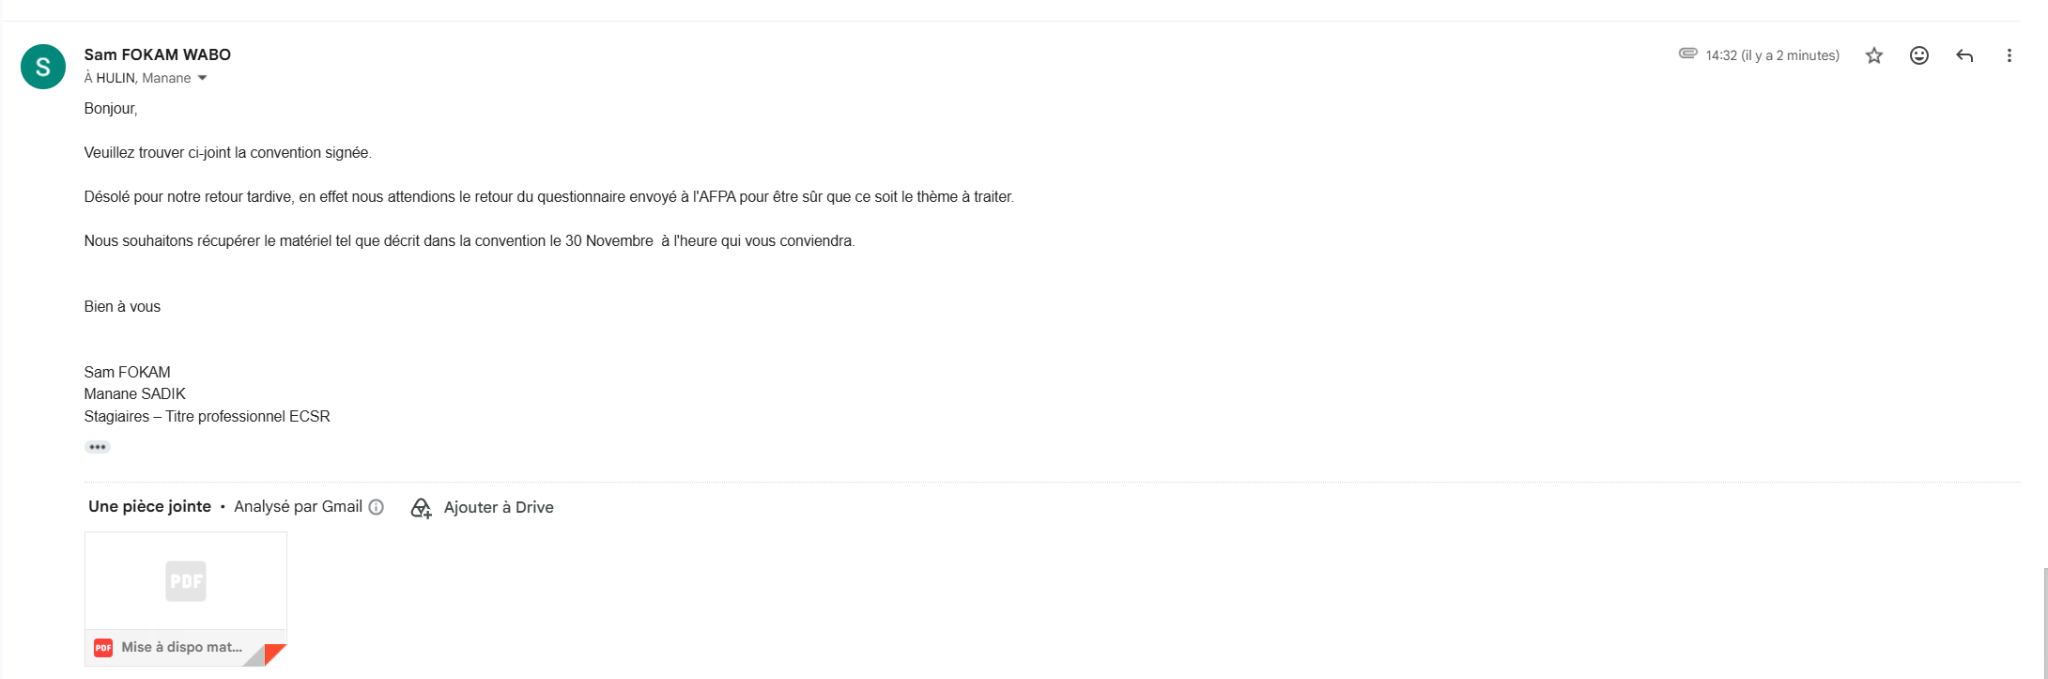
\includegraphics[width=0.97\linewidth,height=0.77\textheight,keepaspectratio]{images/annexes/echanges/p03_20261030_convention_signee.png}
\end{center}
\end{landscape}

\section{Convention et accès logistique au CADAM (A8)}
Échanges relatifs à la signature, aux dates de retrait et de restitution et à la demande d’accès au site. Les opérations effectives restent à confirmer.

\clearpage
\begin{landscape}
\thispagestyle{plain}
\noindent{\large\bfseries 10 novembre — Convention contresignée et changement de retrait}\par\medskip
\begin{center}

\includegraphics[width=0.97\linewidth,height=0.77\textheight,keepaspectratio]{images/annexes/echanges/p04_20261110_convention_prefecture.png}
\end{center}
\end{landscape}

\clearpage
\begin{landscape}
\thispagestyle{plain}
\noindent{\large\bfseries 10 novembre — Accord sur les nouvelles dates}\par\medskip
\begin{center}

\includegraphics[width=0.97\linewidth,height=0.77\textheight,keepaspectratio]{images/annexes/echanges/p05_20261110_confirmation_dates.png}
\end{center}
\end{landscape}

\clearpage
\begin{landscape}
\thispagestyle{plain}
\noindent{\large\bfseries 12 novembre — Précisions des horaires d’accueil}\par\medskip
\begin{center}

\includegraphics[width=0.97\linewidth,height=0.77\textheight,keepaspectratio]{images/annexes/echanges/p06_20261112_plages_horaires.png}
\end{center}
\end{landscape}

\clearpage
\begin{landscape}
\thispagestyle{plain}
\noindent{\large\bfseries 12 novembre — Confirmation de la matinée et du véhicule}\par\medskip
\begin{center}

\includegraphics[width=0.97\linewidth,height=0.77\textheight,keepaspectratio]{images/annexes/echanges/p07_20261112_immatriculation.png}
\end{center}
\end{landscape}

\clearpage
\begin{landscape}
\thispagestyle{plain}
\noindent{\large\bfseries 12 novembre — Demande d’accès annoncée}\par\medskip
\begin{center}

\includegraphics[width=0.97\linewidth,height=0.77\textheight,keepaspectratio]{images/annexes/echanges/p08_20261112_demande_acces.png}
\end{center}
\end{landscape}

\clearpage
\begin{landscape}
\thispagestyle{plain}
\noindent{\large\bfseries 12 novembre — Formalisation de la demande d’accès au CADAM}\par\medskip
\begin{center}

\includegraphics[width=0.97\linewidth,height=0.77\textheight,keepaspectratio]{images/annexes/echanges/p09_20261112_acces_cadam.png}
\end{center}
\end{landscape}

\section{Repères de correspondance avec le CCP2}
\begin{description}[leftmargin=2.9cm,style=nextline]
\item[Compétence 8] Analyse de la demande : prospection, clarification, questionnaire commanditaire et diagnostic du public (chapitres II à IV).
\item[Compétence 9] Construction et préparation : objectifs, moyens, partenaires, scénario et tableau synoptique (chapitre IV).
\item[Compétence 10] Animation de la séance : déroulement effectif et évaluation des acquis (chapitre V, après intervention).
\item[Compétence 11] Analyse de pratique et évolution professionnelle : retour réflexif, remédiations et veille (chapitres VI et VII).
\end{description}

\section{Pièces à intégrer avant remise}
\texteguide{Joindre, dans la version finale uniquement, les pièces autorisées et anonymisées. Privilégier les extraits pertinents : le fichier de réponses individuelles brutes reste un document de travail et n'a pas à être annexé avec ses horodatages.}

\end{document}
